

\section{Applications}

\subsection{CMB data analysis}
\label{sect:NUMEXP}

\index{CMB}
\index{CMB!ICA}
\index{ICA!CMB}

\subsubsection{Introduction}
In modern cosmology, the study of the primordial cosmic microwave background radiation field is one of the major fields of research. 
The reason is the link between CMB properties and the cosmological parameters, CMB existence and properties were predicted by ``Big Bang" theories, and so an 
accurate measurement of the CMB allows constraints on these parameters and discriminations between cosmological models. This great interest is enlightened by 
the number of missions launched in order to increase the accuracy of the measures: spatial mission with COBE~\citep{gauss:smoot92,gauss:kunz01,astro:rocha04} 
in 1990's which has produced the first full-sky maps, Wilkinson Microwave Anisotropy Probe (WMAP)~\citep{astro:bennett2003,astro:2005MNRAS.364.1185P} launched in 2003, 
the last one being the Planck mission launched in june 2009. 
%Other important missions have used stratospherical balloons like Boomerang and Archeops \citep{gauss:fixsen96,gauss:bouchet00,gauss:benoit03}.\\

CMB observation is quite difficult: it is a radiation with very low intensity and even in the best frequency ranges, several signals are recieved together in 
a mixture, making CMB recovery a blind source separation problem or more exactly a semi-blind problem since the contribution of some component is known. Planck mission 
will make sky's observation of high accuracy (a resolution of 5 arcmin for the best observations) in 9 channels whose frequency ranges are going from 30 to 857 GHz.
In that ranges, Planck's instruments will observe several astrophysical components which are summarized in the following list:
\begin{enumerate}
\item {\bf Cosmic Microwave Background:} Towards multichannel modelization, the CMB emission at frequency $\nu$ ${\bf x}_\nu^{cmb}$ is the product of $\Delta T^{cmb}$, 
maps of the fluctuations of CMB (independent of $\nu$) and of an emission law defined as the derived of a blackbody law at CMB temperature ($\bar{T} \simeq 2,735K$):
\begin{equation}
{\bf x}_\nu^{cmb} = \Delta T^{cmb} \left[ \frac{\partial B_\nu(T)}{\partial T} \right]_{T = \bar{T}}
\end{equation}
So the CMB component included in the data $\bf X$ could be modeled as a perfect linear mixture with a known mixing column:
\begin{equation}
{\bf a}^{cmb} = \left[\left[ \frac{\partial B_\nu(T)}{\partial T} \right]_{T = \bar{T}}\right]_{\nu=\left\{\mbox{30,$\cdots$,857GHz}\right\}}
\end{equation}
\item {\bf "Sunyaev Zel'Dovich" effect:} The Sunyaev Zel'Dovich effect is the inverse Compton diffusion of CMB photons with free electrons of a ionized region. 
More precisely, there is two kind of SZ effect:
\begin{itemize}
\item {\bf Thermal SZ effect:} It is linked to photon diffusion in high temperature electron gases such as those in galaxies clusters. In first approximation, thermal SZ 
could be modeled as a linear mixture component:
\begin{equation}
{\bf X}^{sz} = {\bf a}^{sz}{\bf s}^{sz}
\end{equation}
\item {\bf Kinetic SZ effect:} It is linked to the diffusion of photons in an electron gases moving toward CMB. Kinetic SZ has an emission law similar to the CMB one 
but with lower amplitude and so difficult to distinguish from it. It is highly correlated to galaxies clusters and it's estimation could be done as a post-processing 
of the CMB map after source separation.
\end{itemize}
\item {\bf Galactic components:} These components are linked to the milked way emissions:
\begin{itemize}
\item {Synchrotron emission:} This component is created by the move of electric charges particles in a magnetic field. In our galaxy, such effects are intense in 
the galaxy's center but could also takes place in high latitudes. It is modeled as the product of a field with power law signal $\nu^{-\beta}$ for each pixel 
on the sphere. As such it is a non-linear mixture.
\begin{equation}
\forall \nu; \quad { x}_\nu^{sync}[i] = { s}^{sync}[i]\nu^{-\beta^{sync}[i]}
\end{equation}
\item {\bf Free-Free emission:} This component comes from the interaction between free electrons and ions in galactic environment. The energy lost by those interactions 
generates the emission of photons. As a first approximation, the "Free-Free" component could be modeled as a linear mixture, the product of a temperature field and a power 
law signal with spectral index $\beta^{FF} \simeq 2,15$. Thus for frequency $\nu$, the modeling is:
\begin{equation}
\forall \nu; \quad {\bf x}_\nu^{FF} = {\bf s}^{FF}\nu^{-\beta^{FF}}
\end{equation}
\item {\bf Thermal dust emissions:} Several effects may be at the origins of those components. Actually, the description of dust's emissions is only empirical, giving 
the following result for each pixel on the sphere:
\begin{equation}
\forall \nu; \quad {x}_\nu^{D}[i] \propto \frac{\nu^{\beta^D[i]}}{exp(h\nu/k {s}^D[i]) - 1}
\end{equation}
where $\bbeta^D$ is a field of spectral indexes of an emission law and ${\bf s}^D$ is a temperature field. As the synchrotron component, the dust component could not be modeled as a linear mixture.
\end{itemize}
This list of components is not full and some may add extra signals to it.
\end{enumerate}

\subsubsection{Hypothesizes on the mixture model}

As a first approximation, the data are a linear stack of all astrophysical components: 
\begin{equation}
{\bf X} = {\bf X}^{cmb} + {\bf X}^{SZ}  + {\bf X}^{FF} + {\bf X}^{sync} + {\bf X}^{D} + {\bf X}^{PS} + {\bf N}
\end{equation}
Our interest is mainly on the first five components. Except those signals, the data $\bf X$ are corrupted by point sources (infra-red and radio galaxies, quasars, etc\ldots) 
${\bf X}^{PS}$, each one with its own emission law. Clearly ${\bf X}^{PS}$ is not a rank $1$ matrix. $\bf N$ modelizes intrumental noise.

Each of these components has its own interest for astrophysicians' working groups. For us, our interest is the CMB map and the computation of its power spectrum. 
We have chosen to apply GMCA algorithm in order to extract the map of temperatures' fluctuations of the CMB ${\bf s}^{cmb}$. An accurate estimation of the CMB 
requires an efficient decomposition of the input data, thus the joint estimation of the greatest number of galactical components.

For the separation processing, the major problem comes from the components "Dust" and "Synchrotron" which could act quite non-linearly in the mixture. A first approach is 
to neglect this and consider that those signals behave like linear mixture:
\begin{eqnarray}
{\bf X}^{sync} & = & {\bf a}^{sync} {\bf s}^{sync}\\
{\bf X}^{D} & = & {\bf a}^{D} {\bf s}^{D}
\end{eqnarray}
This approximation is simple and could be considered as acceptable on some part of the sphere (especially in high latitudes sections, far from galaxy plane). The non-linear caracteristic 
(for the mixing) of "Dust" and "Synchrotron" components is to some extent linked to the fluctuations of $\bbeta^{sync}$, $\bbeta^{D}$ and ${\bf s}^{D}$. It seems that the fluctuations of 
those fields are limited and slow for part of the sky far from the galactic center. On such parts, the linear mixture model is true as a first approximation.

ESA/Planck consortium has implemented several working groups, one of them (WG2) dedicated to the source separation. Inside WG2, sources separation experiments are run on realistic 
synthetic data expected closed to those that will be given by Planck's instruments. In the following section, we apply GMCA on such synthetic data.

\subsubsection{Planck/CH2 data}

\paragraph*{data and instrumental limits}

It is the simulated data that were created for the second set of sources separation experiments in 2007 and 2008 (Challenge-2). These data are the 9 Planck channels in the frequency bands: 
$30$, $44$, $70$, $100$, $143$, $217$, $353$, $545$ and $857$ GHz. The observations are those that are expected to be given by Planck consortium after one year of work. Each observation is 
a spherical map sampled with pixelization HEALPix. The total number of pixel per channel is $t = 50331648$. The $9$ Planck channels are thus giving a very huge data set with around $450$ million of pixels. 
The effects of instruments on the data, normalized for WG2/CH2, are the following:
\begin{itemize}
\item {\bf Non-correlated and non-stationnary instrumental noise:} The instrumental noise for a skymap reconstructed after one year observations is linked to the sky scanning process. 
More precisely, for a pixel $k$ in channel $i$, the contribution ${\bf N}[i,k]$ will have a variance proportionnal to the invert of the number of time where the corresponding area of 
the sky would have been scanned. In first approximation, the noise will be considered as gaussian, with zero mean and such as:
\begin{eqnarray}
\forall i \mbox{ et } k \neq k^\prime; \quad \mathbb{E}\left\{{\bf N}[i,k] {\bf N}[i,k^\prime ] \right\} &=& 0\\
\forall k \mbox{ et } i \neq i^\prime; \quad \mathbb{E}\left\{{\bf N}[i,k] {\bf N}[i^\prime,k ] \right\} &=& 0\\
\forall k \mbox{ et } i; \quad \mathbb{E}\left\{{\bf N}[i,k] ^2\right\}  &=&  \sigma_{{\bf N}i,k}^2
\end{eqnarray}
where $\sigma_{{\bf N}i,k}^2$ is the real noise variance of pixel $k$ in channel $i$. Being linked to the instrument and the scanning of the sky by the sattelite, this real variance is known.\\
\item {\bf Resolution and convolution:} The sky is observed by Planck in several frequency bands. The instrument's aperture being fixed, each channel thus has its own spatial resolution. 
The table~\ref{table_res_list} gives the resolution of each channel (in arcminute). The circular aperture of the instrument being finite, it is equivalent to consider that the data are convolved 
with a gaussian kernel whose half-height width is the resolution of the instrument.
\begin{center}
\begin{table}[h!b!p!]
\begin{center}
{\begin{tabular*}{0.95\textwidth}{@{\extracolsep{\fill}}|c||c|c|c|c|c|c|c|c|c|}
\hline
\hline  % put a line under headers
Channel (in GHz) & $30$  & $44$ & $70$  & $100$  & $143$ & $217$ & $353$  & $545$  & $857$\\
\hline
Resolution (in arcminute) & $33$  & $24$ & $14$  & $10$  & $7$ & $5$ & $5$  & $5$  & $5$\\
\hline
\end{tabular*} }
\caption{\textbf{Spatial resolution per channel } \label{table_res_list}}
\end{center}
\end{table}
\end{center}
In the given simulations, the convolution kernel is isotropic and fully known.\\
\end{itemize}
Each real observation ${\bf y}_i$ could be modelled as:
\begin{equation}
\forall i=1,\cdots,m; \quad {\bf y}_i = \left( {\bf h}_i \star {\bf x}_i\right) + {\bf n}_i
\end{equation}
where ${\bf x}_i$ is the perfect observation for channel $i$: without convolution and noise. ${\bf h}_i$ is the convolution kernel for channel $i$. The data $\bf Y$ of WG2/CH2 could be shown 
on the Figure~\ref{fig:data_wg2}.

\begin{figure}[htb]
\vfill
\hspace{0.1in}
\begin{minipage}[b]{0.5\linewidth}
    \centerline{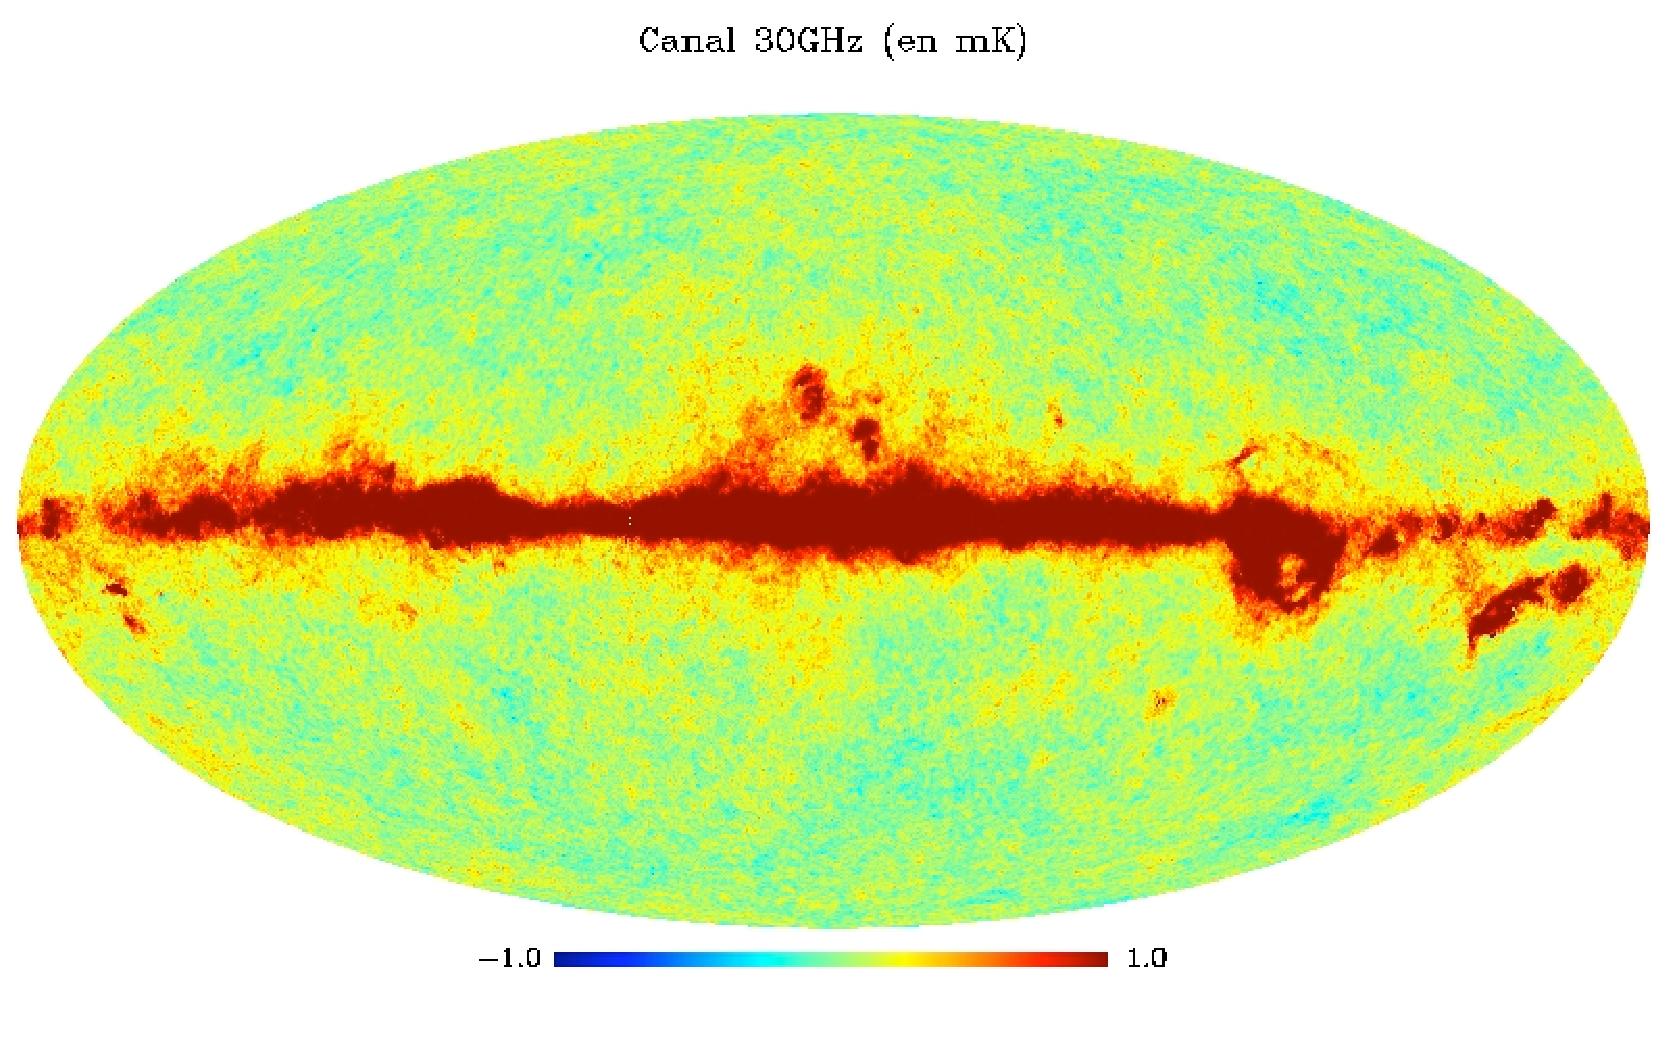
\includegraphics[width=6cm]{input30Ghz.pdf}}
\end{minipage}
\hfill
\begin{minipage}[b]{0.5\linewidth}
    \centerline{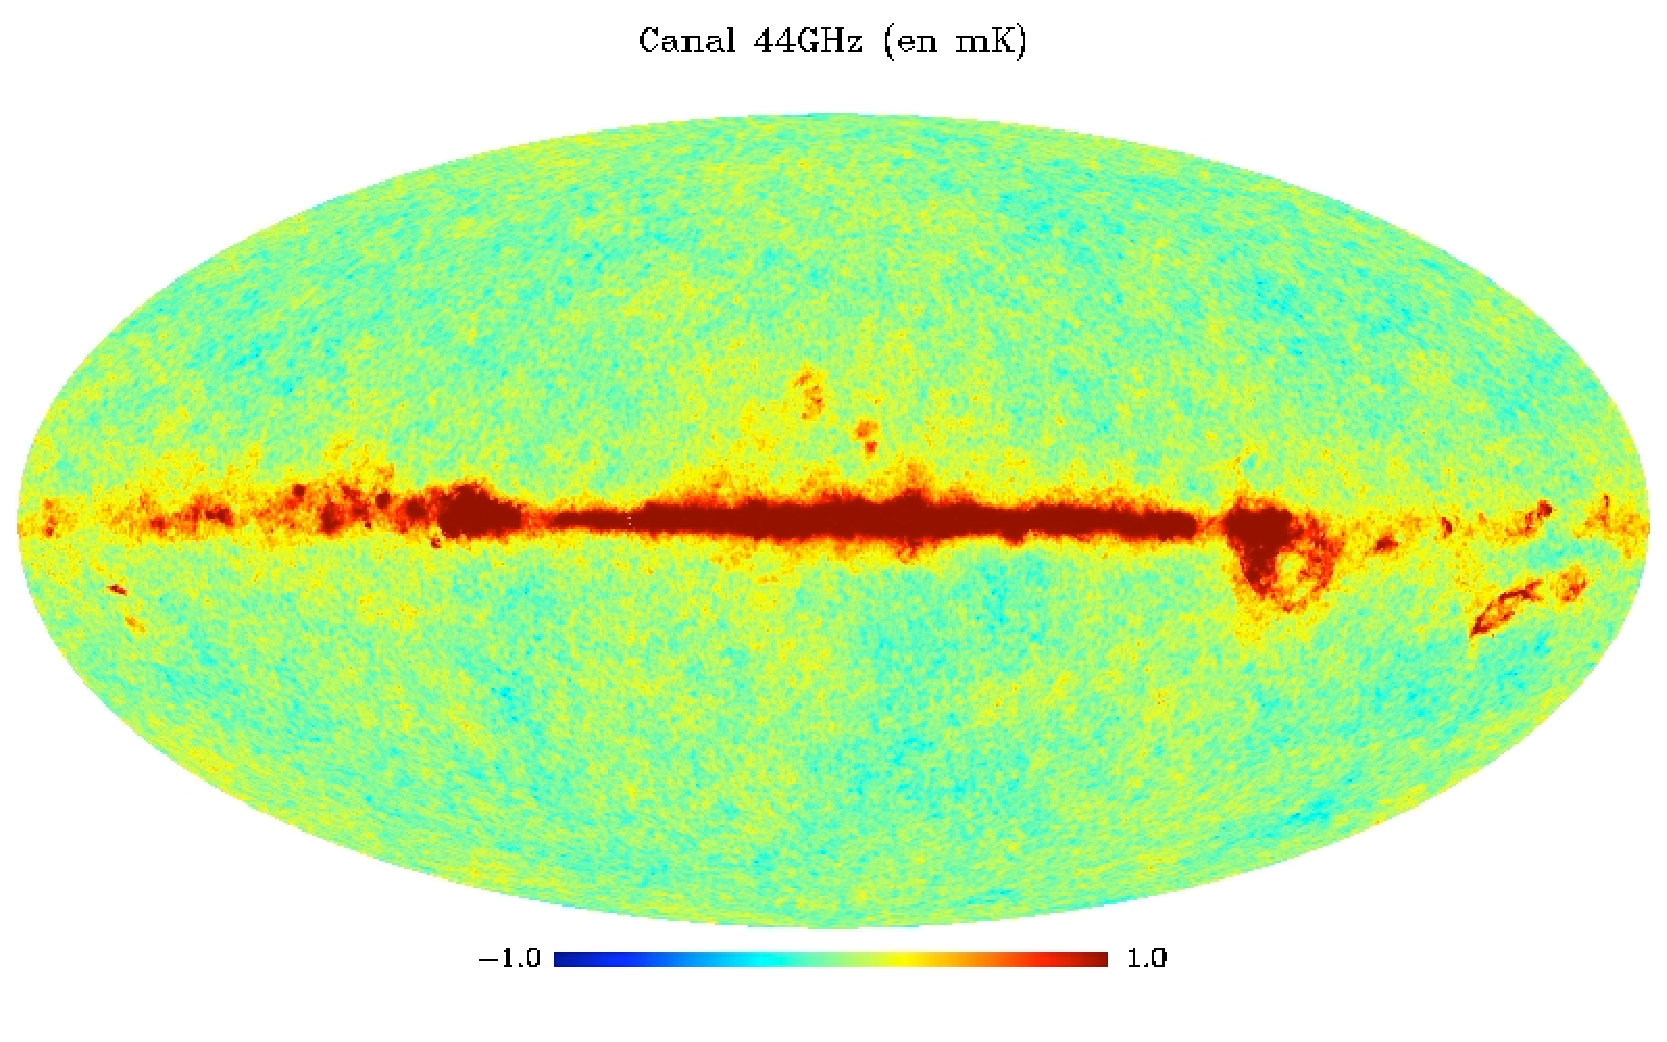
\includegraphics[width=6cm]{input44Ghz.pdf}}
\end{minipage}
\vfill
\hspace{0.1in}
\begin{minipage}[b]{0,5\linewidth}
    \centerline{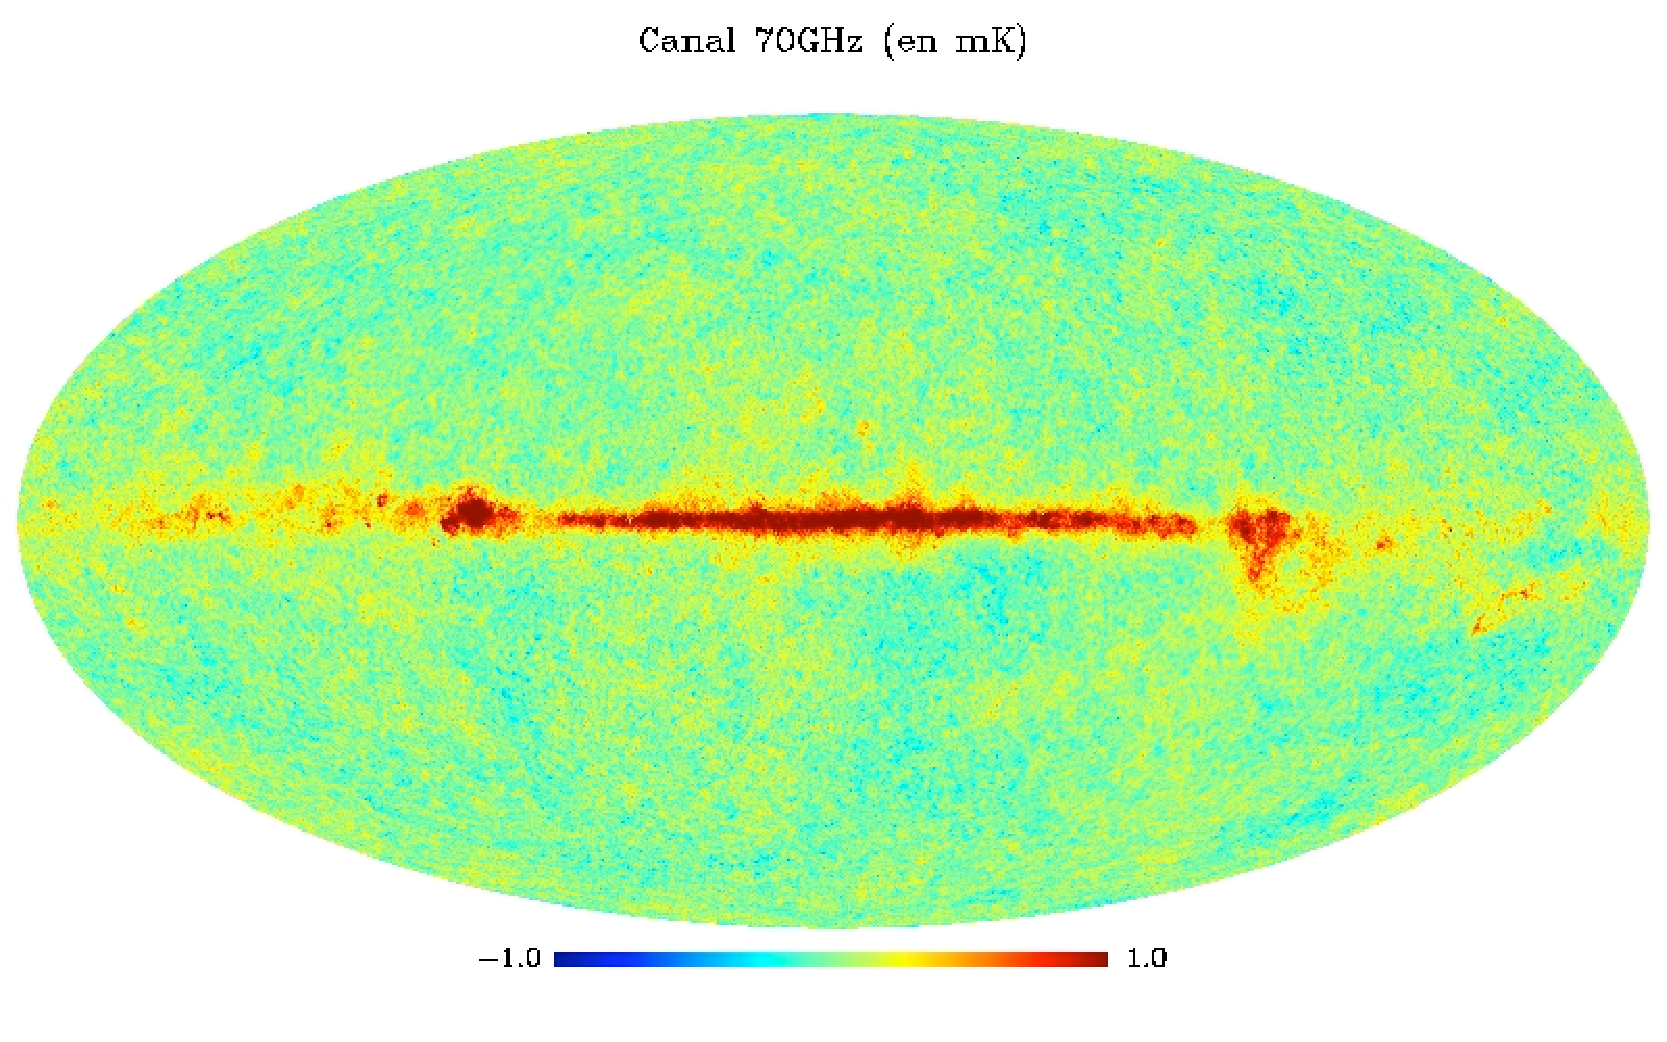
\includegraphics[width=6cm]{input70Ghz.pdf}}
\end{minipage}
\hfill
\begin{minipage}[b]{0,5\linewidth}
    \centerline{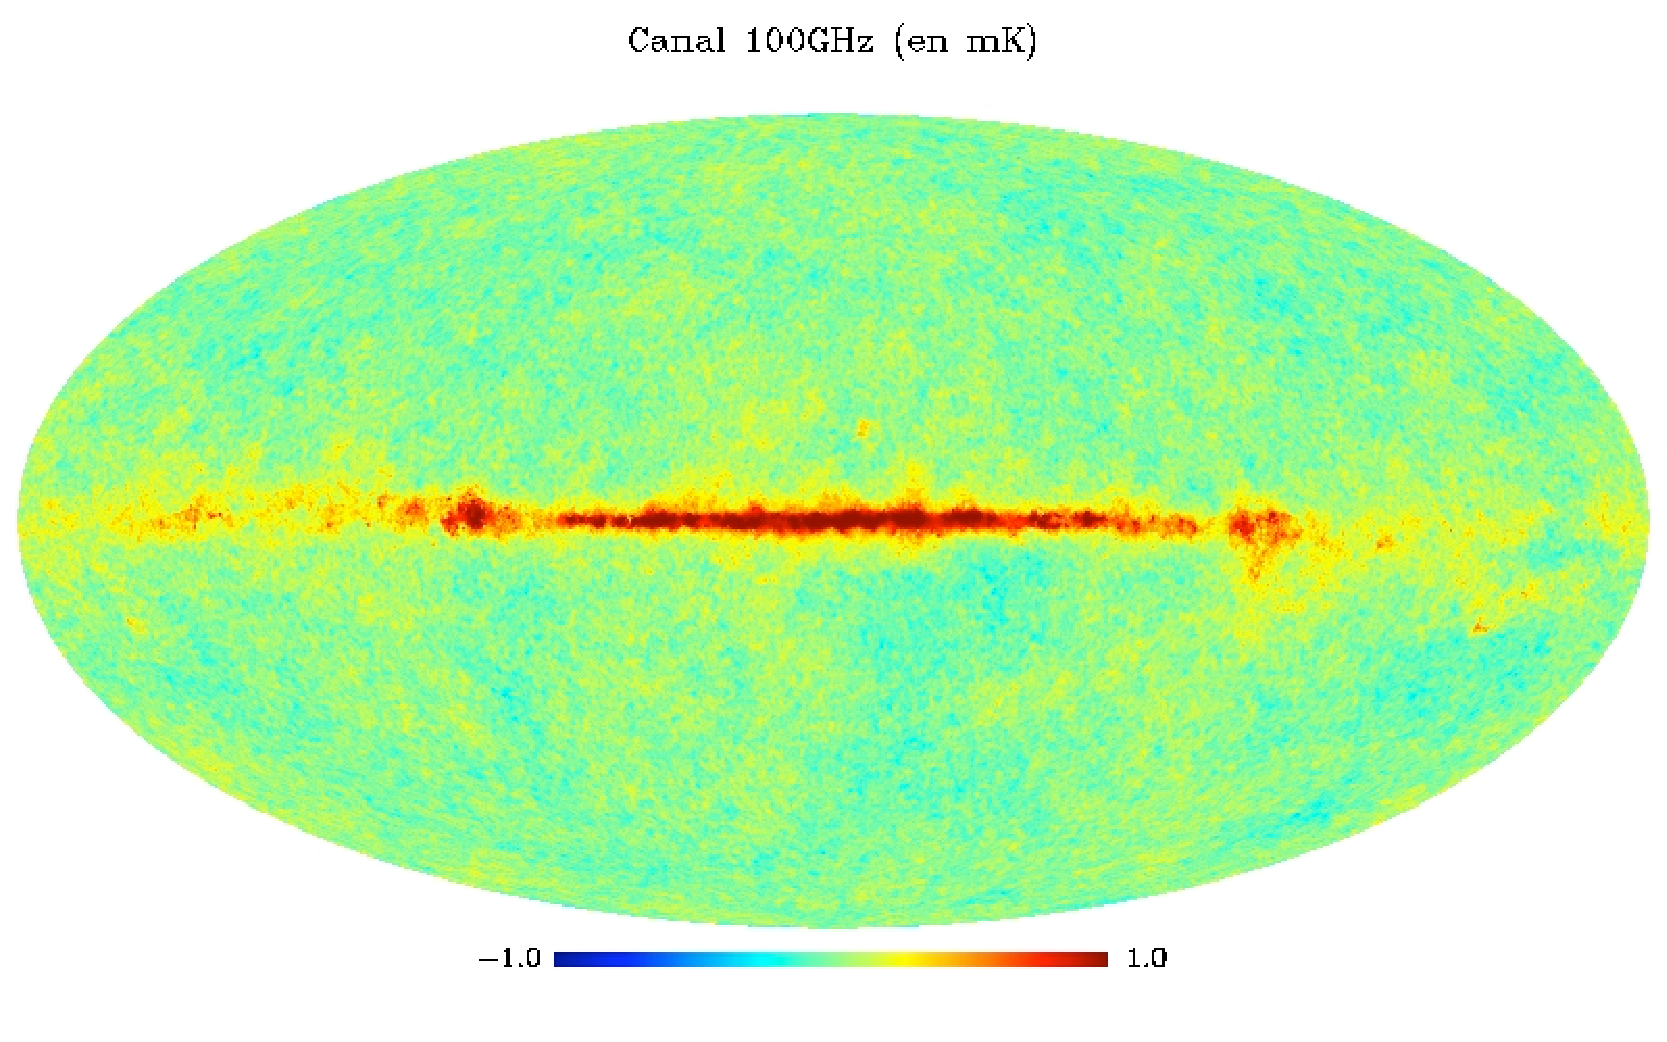
\includegraphics[width=6cm]{input100Ghz.pdf}}
\end{minipage}
\vfill
\hspace{0.1in}
\begin{minipage}[b]{0,5\linewidth}
    \centerline{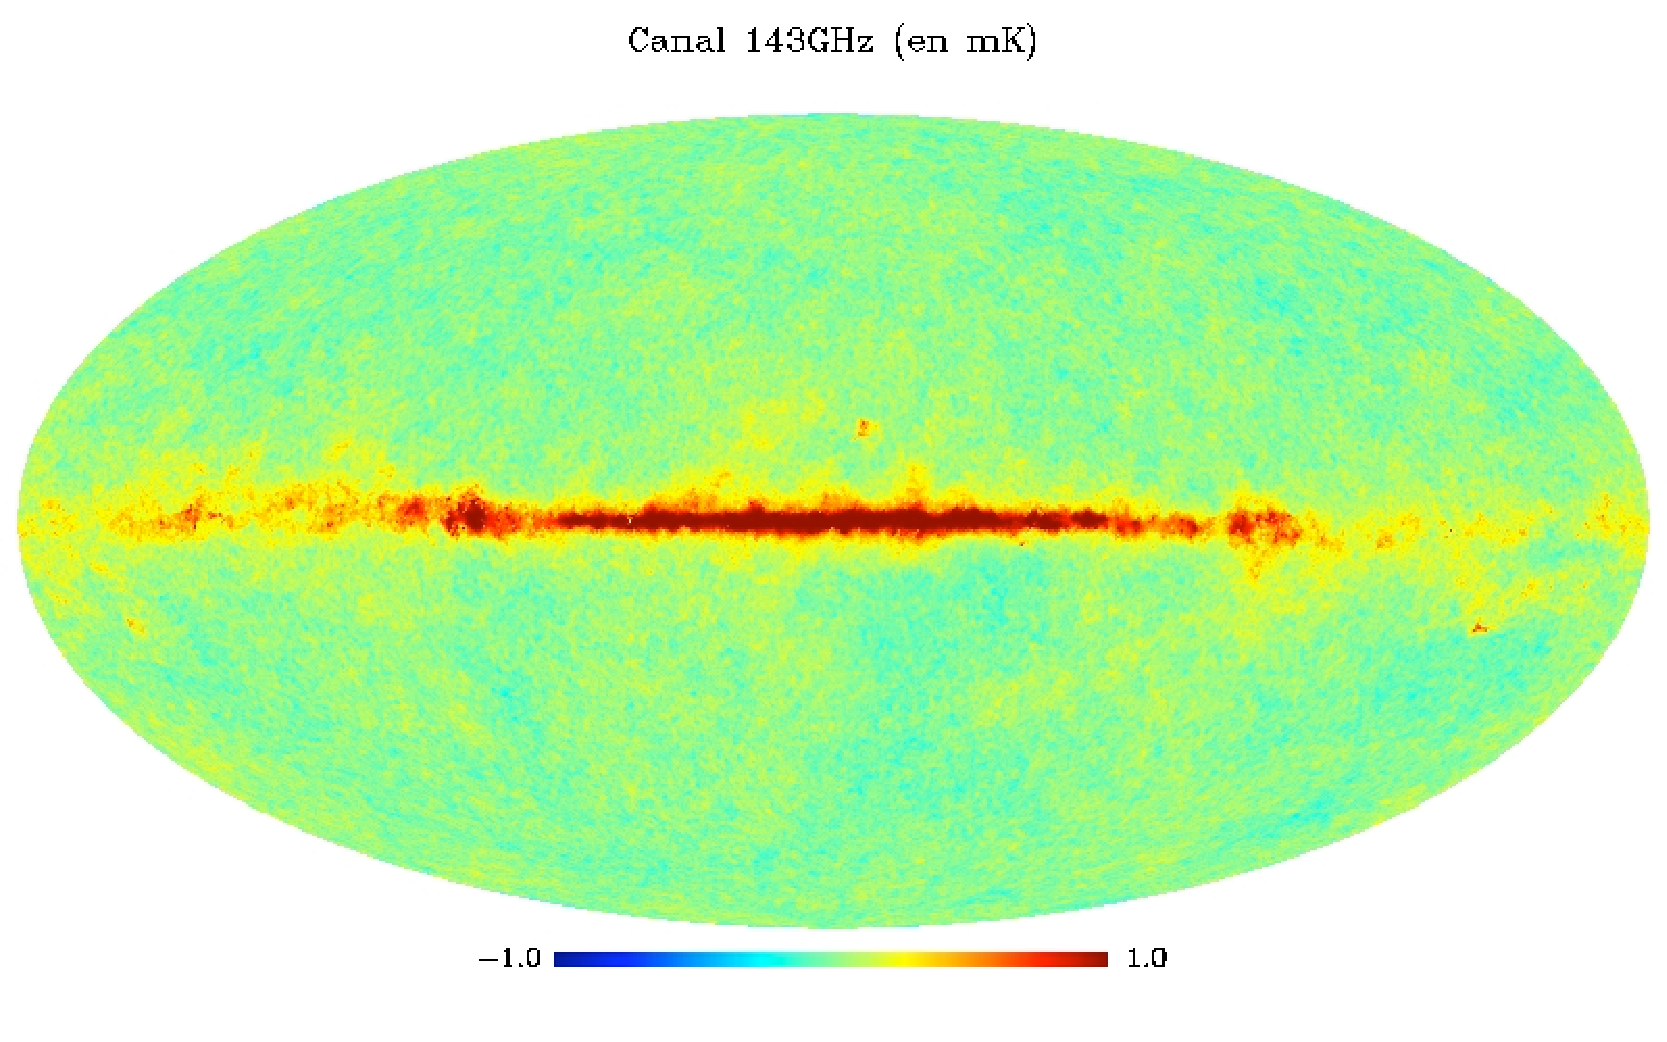
\includegraphics[width=6cm]{input143Ghz.pdf}}
\end{minipage}
\hfill
\begin{minipage}[b]{0,5\linewidth}
    \centerline{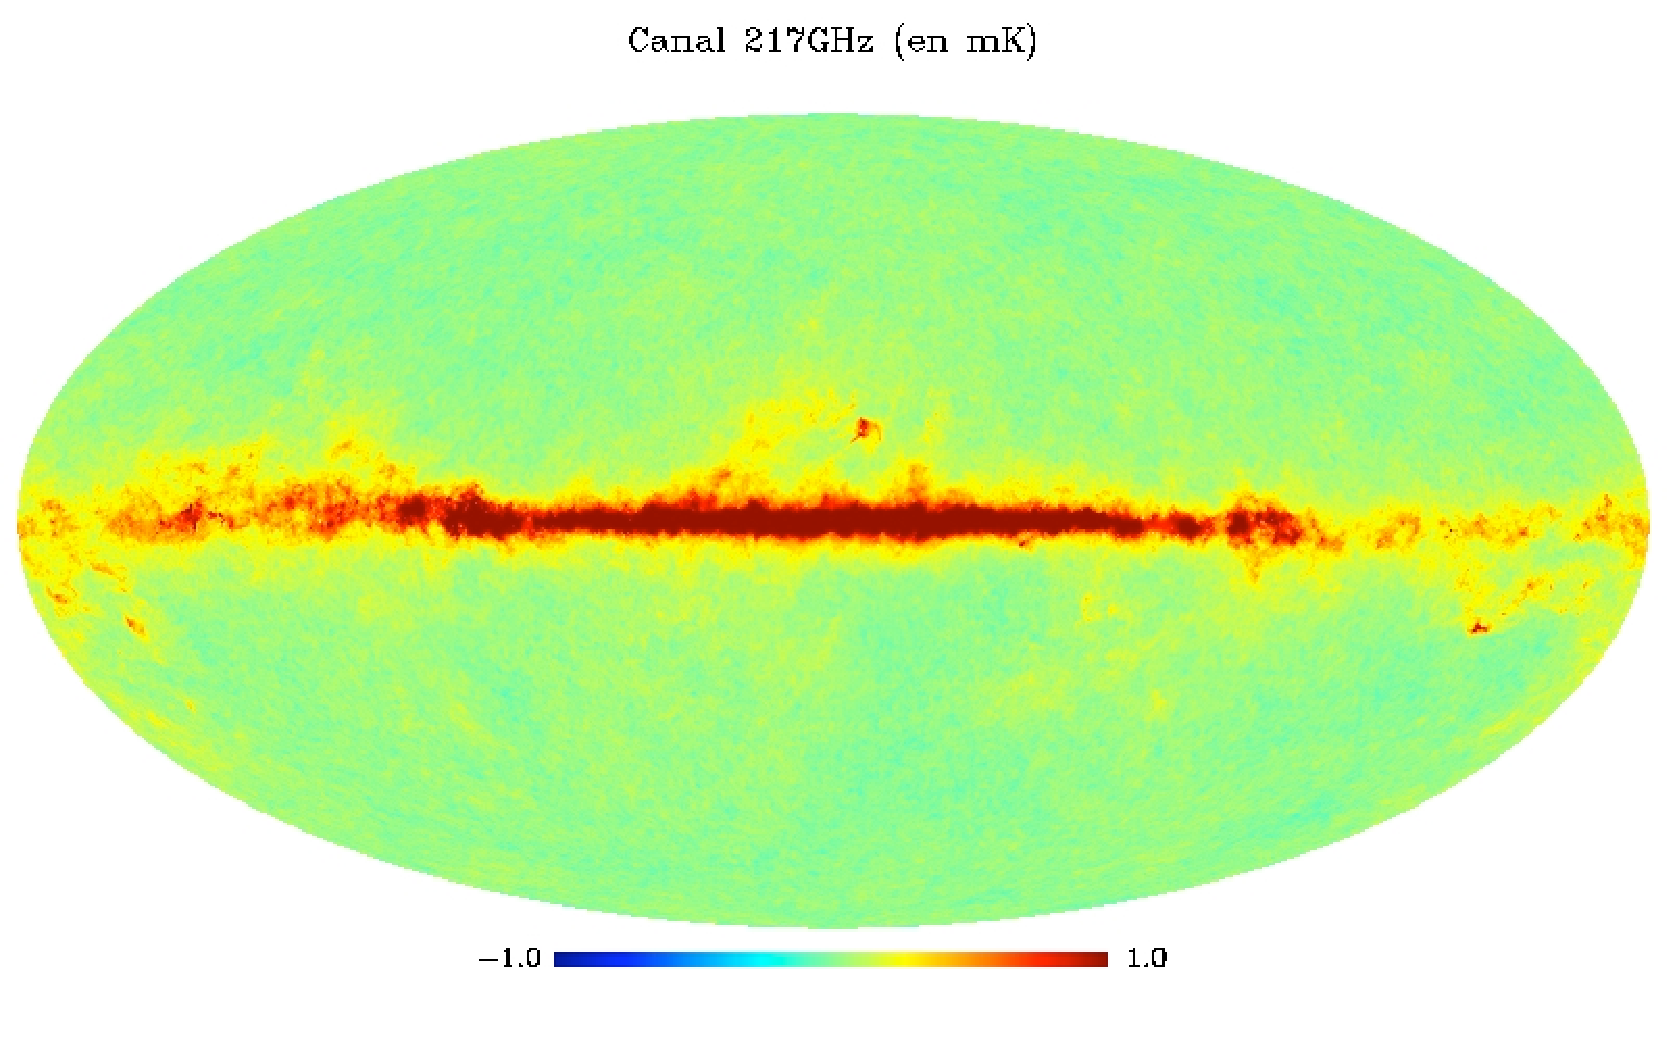
\includegraphics[width=6cm]{input217Ghz.pdf}}
\end{minipage}
\vspace{-0.1in} 
\vfill
\hspace{0.1in}
\begin{minipage}[b]{0,5\linewidth}
    \centerline{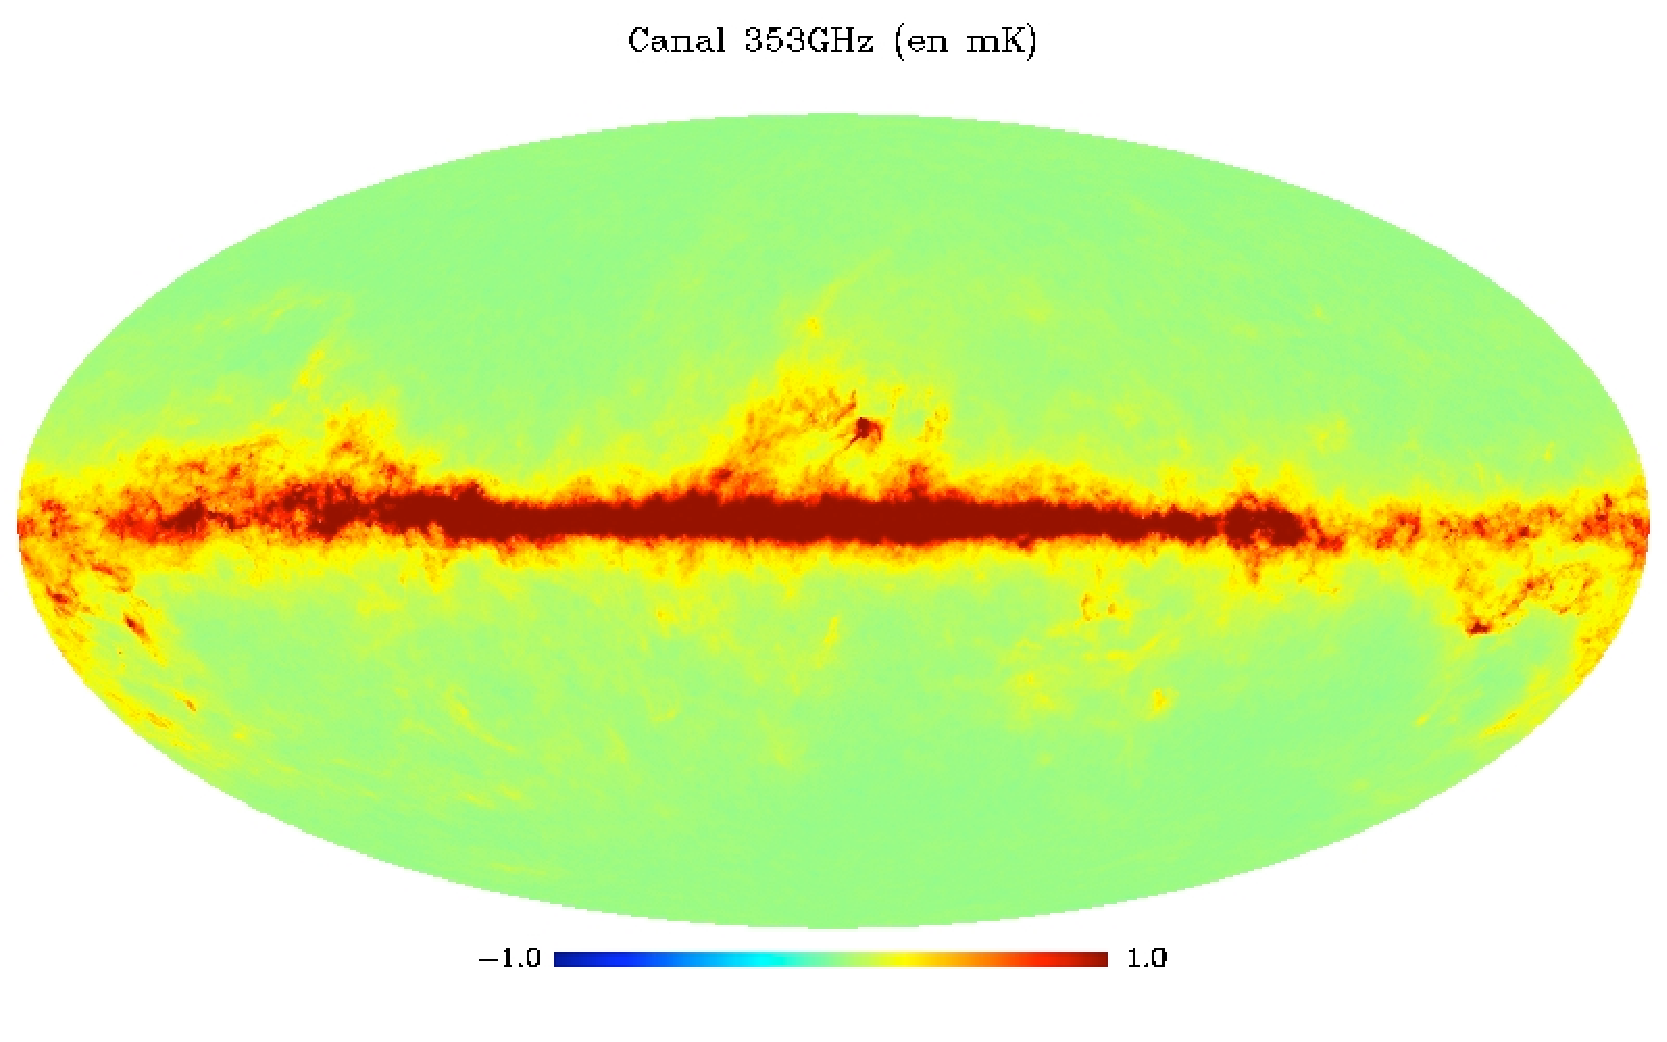
\includegraphics[width=6cm]{input353Ghz.pdf}}
\end{minipage}
\hfill
\begin{minipage}[b]{0,5\linewidth}
    \centerline{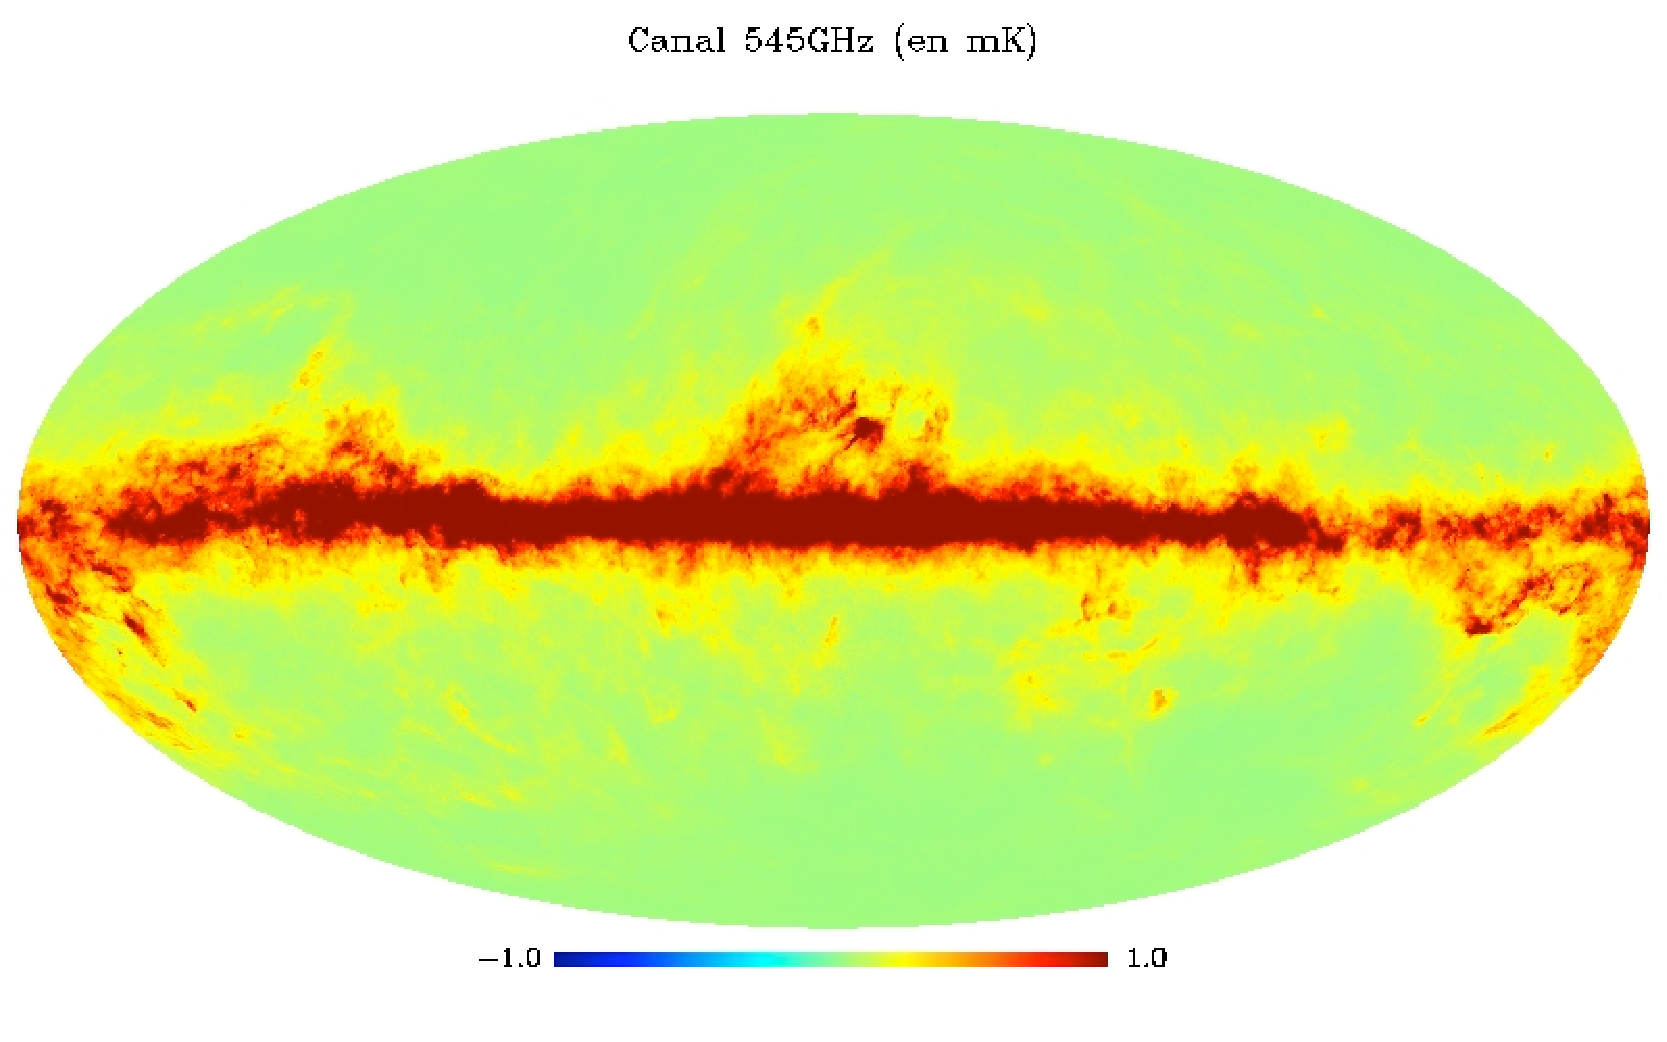
\includegraphics[width=6cm]{input545Ghz.pdf}}
\end{minipage}
\vspace{-0.1in} 
\vfill
\begin{minipage}[b]{1\linewidth}
    \centerline{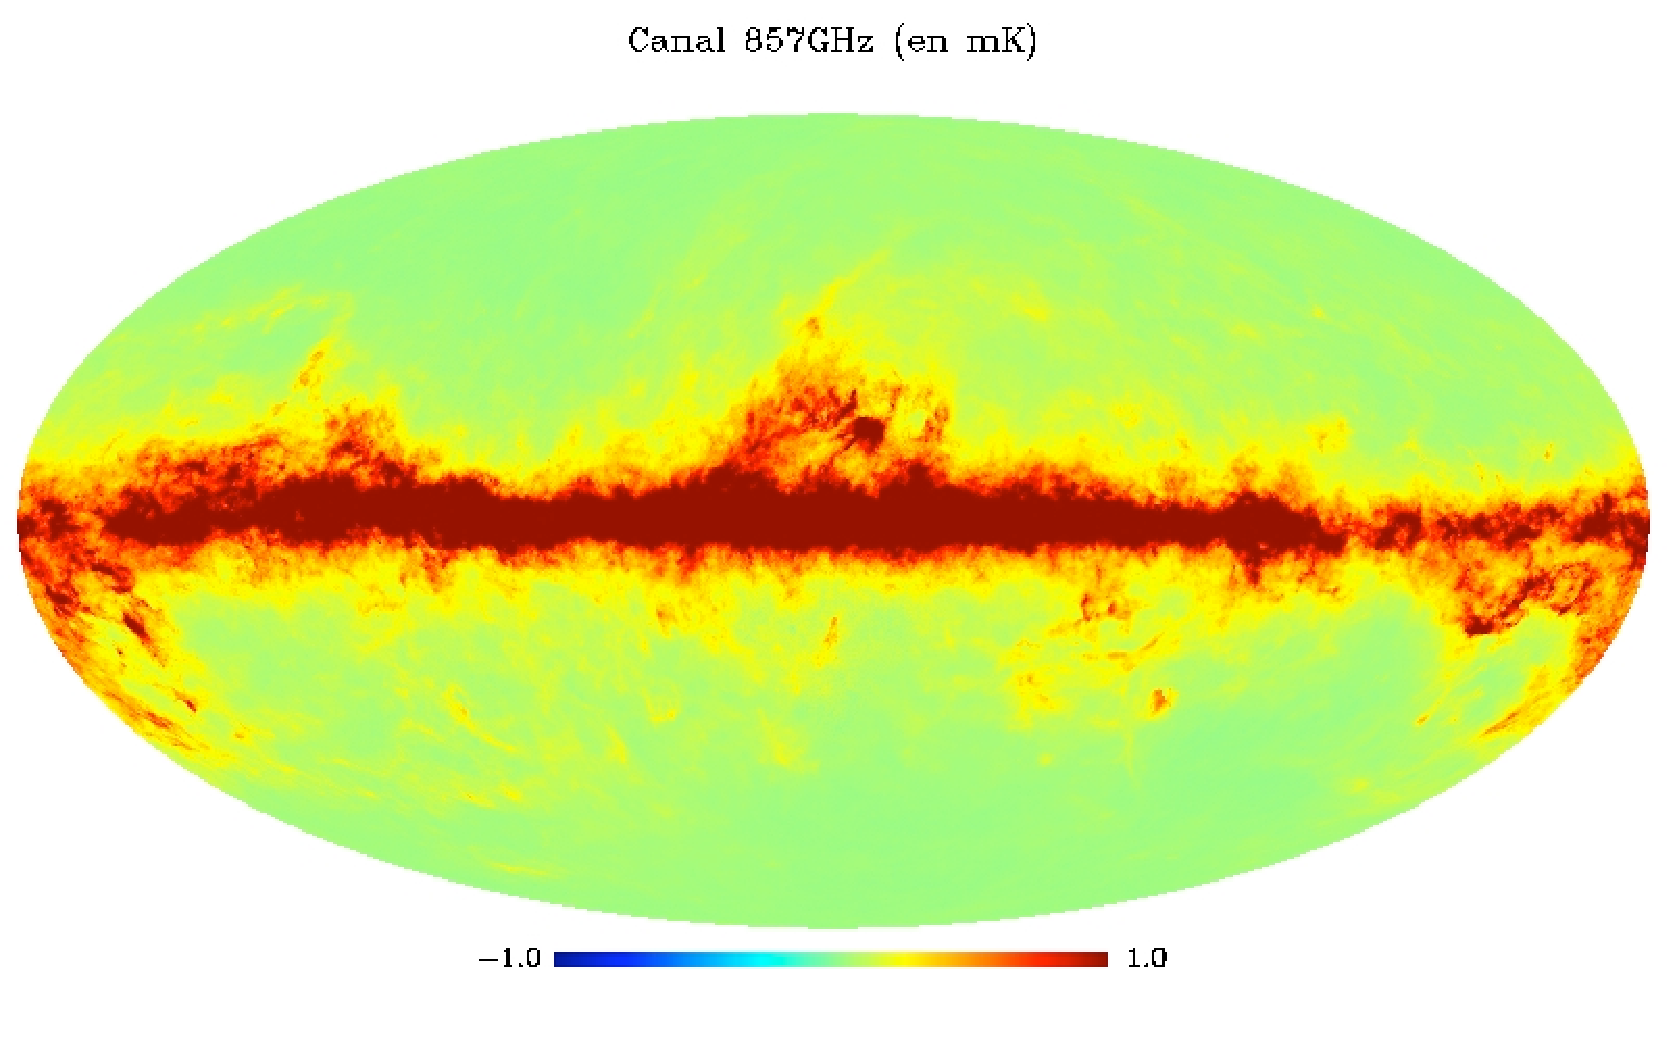
\includegraphics[width=6cm]{input857Ghz.pdf}}
\end{minipage}
\vspace{-0.1in} 

\caption{WG2/CH2 data.}  \label{fig:data_wg2}
\end{figure}

\paragraph*{Physical model for GMCA}

Astrophysical components in the simulated data WG2/CH2 are the folowing:\\
\begin{itemize}
\item {\bf CMB:} The only hypothesis made will be the blackbody spectrum at $2,375\,^\circ K$. The CMB column in the mixing matrix $\bf A$ will be fixed.
\item {\bf SZ:} With a point of view similar to the one used for the hypotheses on the CMB, the linear mixing model of SZ in the frequency ranges observed by Planck is checked well. 
More, the spectral behaviour of SZ is well-known. The SZ column in the mixing matrix $\bf A$ will also be considered known and so fixed.
\item {\bf "Free-Free":} In first approximation, the linear mixing model is checked for the component "Free-Free". Its spectral behaviour is the one of a power law with 
spectral index $\beta^{FF} \simeq 2,15$ \citep{Delabrouille:2005dn}.
\item {\bf "Synchrotron":} Physical models are expecting the synchrotron emissions to have a spectral behaviour like a power law with spatial evolution. The linear mixture model 
is no longer valid. In \citep{Bonaldi:2006fu} it has been proposed to approximate the synchrotron's behaviour as a linear mixture whose spectral index is to be estimated. This hypothesis 
should be accurate for the large scale structures of the synchrotron. More, in \citep{Haslam:1982dk} a synchrotron map with a resolution closed to a quarter of Planck's one have been proposed. 
Our idea is to add an estimation step in the algorithm GMCA in which the spectral index $\beta^{sync}$ will be estimated with a residual cube ${\bf R} = {\bf X} - \sum_{i \neq sync} {\bf a}^i {\bf s}_i$ 
and with the low resolution synchrotron map ${\bf s}_{Haslam}$. $\beta^{sync}$ estimation is done with signals with same resolution (the Haslam map's one) in the following way:
\begin{equation}
\beta^{sync} = \Argmin{\beta} \left\|{\bf R} - {\bf a}^{sync}\left(\beta\right) {\bf s}_{Haslam} \right\|_F
\end{equation}
\item {\bf "Dust":} Thermal dust component is a non-linear mixture. This is the most complex component to modelize since she requires two set of parameters (temperature and spectral index), 
both having spatial variations. Fortunatly, CMB and dust have opposite spectral behaviour: CMB is dominant in low frequency channels whereas dust dominates in high frequency channels. Moreover, 
dust component is highly structured with a sparse decomposition in wavelets. GMCA being built to be sensible to that kind of component, it seems acceptable to recover the dust component 
(or perhaps we should speak of components) blindly.
\item {\bf Point sources:} Infra-red or radio point sources each have their own spectrum. They are more an annoying component towards the goal of extracting diffuses components like CMB. 
Their detection is one of the troubles discovered during the processing of the data (see~\citep{leach08}). After their detection they are often masked.
\end{itemize}

\paragraph*{GMCA algorithm for Planck}

The linearity of BSS model has a major advantage as soon as physical parameters' estimation is needed: for example, once you know the noise's statistical properties on the data, 
the linearity of the model allows to get the noise's statistical properties of the sources in an easy way.The GMCA's version described here considers WG2/CH2 data as a linear 
mixture of components. Beyond the algorithms \ref{algo_gmca} and \ref{algo_fast_gmca} already described, GMCA method is itself ready to include the physical constraints described above.

For the linear mixture model, each observation $\{{\bf x}_i\}_{i=1,\cdots,m}$ could be written as the linear combination of $n$ components. The observed data, including convolution, 
are thus defined in the following way:
\begin{eqnarray}
\forall i=1,\cdots,m; \quad {\bf y}_i &  = & ({\bf h}_i \star {\bf x}_i) + {\bf n}_i \\
& = &  \sum_{j=1}^n A[i,j] ({\bf h}_i \star {\bf s}_j) + {\bf n}_i
\end{eqnarray}
The mixture model is no longer linear towards the observed data $\bf Y$\footnote{It is a non linearity in the sense of the mixing model, the model remains linear in common sense since it is defined as the composition of linear operators.}. Two solutions could be considered: a strict one will the deconvolution of each observation before applying GMCA.
\begin{itemize}
\item {\bf Deconvolution of the data:} A deconvolution is done to each observation. The data having an interchannel structure, a separate deconvolution of each channel is unsuitable. 
Regardless of these considerations, some convolution kernels (especially for low frequecy channels) are leading to an ill-conditioned deconvolution.
\item {\bf Adapt GMCA to joint deconvolution:} GMCA algorithm relies on the iterative estimation of sources and mixing matrix. A deconvolution could be intergrated to 
the sources estimation step for fixed $\bf A$.
\end{itemize}
Due to the really huge size of the data, we have first chosen to apply GMCA to the data $\bf Y$. A compensation of the convolution is then done on the estimated CMB map. In first approximation, 
the most significant diffused structures in the data are dominated by their lowest frequencies for which the convolution operator has the less impact. This point allows us to justify the estimation 
of the mixing matrix $\bf A$ from the data $\bf Y$.

The GMCA method adapted for the processing of Planck data is described in Algorithm~\ref{algo_planck_gmca}.
{\linespread{1}
\begin{algorithm}[htb]
\caption{Planck GMCA algorithm.}
\label{algo_planck_gmca}
\noindent{\bf Task:} Separation of Planck data with GMCA.\\
\noindent{\bf Parameters:} The data $\bf Y$, number of iterations $P_{\max}$, number of sources $N_s$ and channels $N_c$, dictionnary ${\bf \Phi}$, 
mixing matrix $\bf A$ with fixed column setted, initial threshold $\gamma^{(0)}$ stopping threshold ${\gamma_{\min}}$.\\
\noindent{\bf Initialization:} 
\begin{itemize}
\item Set set number of iterations $P_{\max}$ and the initial threshold $\gamma^{(0)}$.
\item Computes a wavelet transform on the sphere of the data ${\bf \balpha_Y}$.\\
${\bf \balpha_Y} = {\bf Y} {\bf \Phi}^T$
\end{itemize}
\noindent{\bf Main iteration:} \\
\While{ Threshold $\gamma^{(h)} > \gamma_{\min}$ (\textit{e.g.} depends on the noise variance)}{
\begin{itemize}
\item Estimation of the sources ${\bf \balpha_S}$ at iteration $h$ with matrix $\bf A$ supposed fixed:\\
${\bf \balpha_{S}}^{(h+1)} = \mathcal{H}_{\gamma^{(h)}}\left({\bf A^\dagger}^{(h)}{\bf \balpha_Y}\right)$
\item Update the free column of the mixing matrix $\bf A$ noted ${\bf A^\circ}$ with ${\bf \balpha_S}$ supposed fixed:\\
${\bf \tilde{A^\circ}}^{(h+1)} = {\bf \balpha_Y}{\bf \tilde{\balpha^\circ}_S}^{{(h)}^T} \left({\bf \tilde{\balpha^\circ}_S}^{{(h)}}{\bf \tilde{\balpha^\circ}_S}^{{(h)}^T}\right)^{-1}$
\item Estimation of synchrotron's spectral index $\beta^{sync}$ from the residual ${\bf \balpha_R} = {\bf \balpha_Y} - \sum_{i \neq sync} {\bf a}^i {\bf \balpha_{S}}_i$:\\
$\beta^{sync} = \Argmin{\beta} \left \| {\bf \balpha_R} - {\bf a}^{sync} {\bf \balpha}_{Haslam} \right \|_2$
\item Update the synchrotron column of $\bf A$
\item Decrease the threshold $\gamma^{(h)}$.
\end{itemize}
}
\noindent{\bf Output:} Estimated mixing matrix ${\bf \tilde{A}}^{(\niter)}$.
\end{algorithm}}

\subsubsection{Results}

Most of the results are for the estimation of the CMB map. The figure~\ref{fig:wg2_maps} gives the initial simulated CMB map (top) and the one estimated with GMCA (bottom). 
A remark is that GMCA estimates a miximg matrix $\bf A$ used to estimate a noisy CMB map by applying the pseudo-invert of $\bf A$ to the data $\bf Y$. In the hypothesis of 
a perfect separation of the components, the estimated CMB map is isotropic and so characterized only by its power spectrum. Convolution of the data lead to a power loss that 
could be corrected by the computation of a filter determined with the convolutions' kernels $\{{\bf h}_i\}_{i=1,\cdots,m}$ and the mixing matrix $\bf A$. The denoising of 
the CMB map is then done with a Wiener filtering in the spherical harmonics space. The map estimated by GMCA in figure~\ref{fig:wg2_maps} is this map obtained after Wiener filtering. 
It is well known that Wiener filtering induces a biais all the more important so SNR is low. In first approximation, the noise's spectrum is flat (stationnary in spherical harmonics space). 
The spatial spectrum of the CMB has a decreasing in the range of $1/\ell$, thus the biais on the filtered component will be greater for high $\ell$ values. This explains the differences 
between the original map and the estimated CMB map which shows a loss in high frequency structures (high $\ell$ values) on the estimated map.

In order to precisely analyze the estimated map, a solution is to observe the residual ${\bf r}_{CMB} = {\bf s}_{CMB} - {\bf \tilde{s}}_{CMB}$ (between the input map and the estimated map) 
convolved by a gaussian beam, which allows the a more suitable estimation of large structures (low $\ell$ values). Here we make comparisons between the map estimated with GMCA and maps 
estimated by the groups ADAMIS, CCA and MEM whose methods could be found in \citep{leach08}. The residual convolved with a gaussian kernel of $20$ arcminutes (which corresponds to a 
half-height width of $\ell = 500$) are given in figures~\ref{fig:wg2_resi20} and \ref{fig:wg2_resi20_2}. At first sight, the high latitudes residual (out of galactic center) seems limited 
compared to the other results. Galactic center mainly shows a residual of galactic dust. Figures~\ref{fig:wg2_resi60} and \ref{fig:wg2_resi60_2} are the same residuals but convolved this time 
with a gaussian kernel of $60$ arcminutes (which corresponds to a half-height width of $\ell = 180$). The observation of this convolved residual mainly show the really large structures. 
It corroborates the   observations made from the residual convolved at $20$ arcminutes: GMCA with physical constraints is able to recover a CMB component whose large scales are preserved 
out of the galactic center.

Figure~\ref{fig:wg2_resiperlat} shows the standard deviation of the residual convolved at $20$ (top) and $60$ (bottom) per latitude bands with a width of $20^\circ$. The value $90^\circ$ corresponds 
to the galactic center and since this band is highly corrupted by galactic components, the corresponding result is not plotted. The bottom plot for the residual, convolved at $60$ arcminutes seems, to 
corroborate the good results of GMCA outside the galactic center. Strangely the result is slightly different for the residual convolved at $20$ arcminutes scince it shows a lower residual for ADAMIS. 
It seems that this is due to a diredt compensation of deconvolution. This latter one leads to create \textit{ringing} artefact araound residual structures of point sources or galactical components.

\begin{center}
\begin{figure}[htb]
$$
\begin{array}{cc}
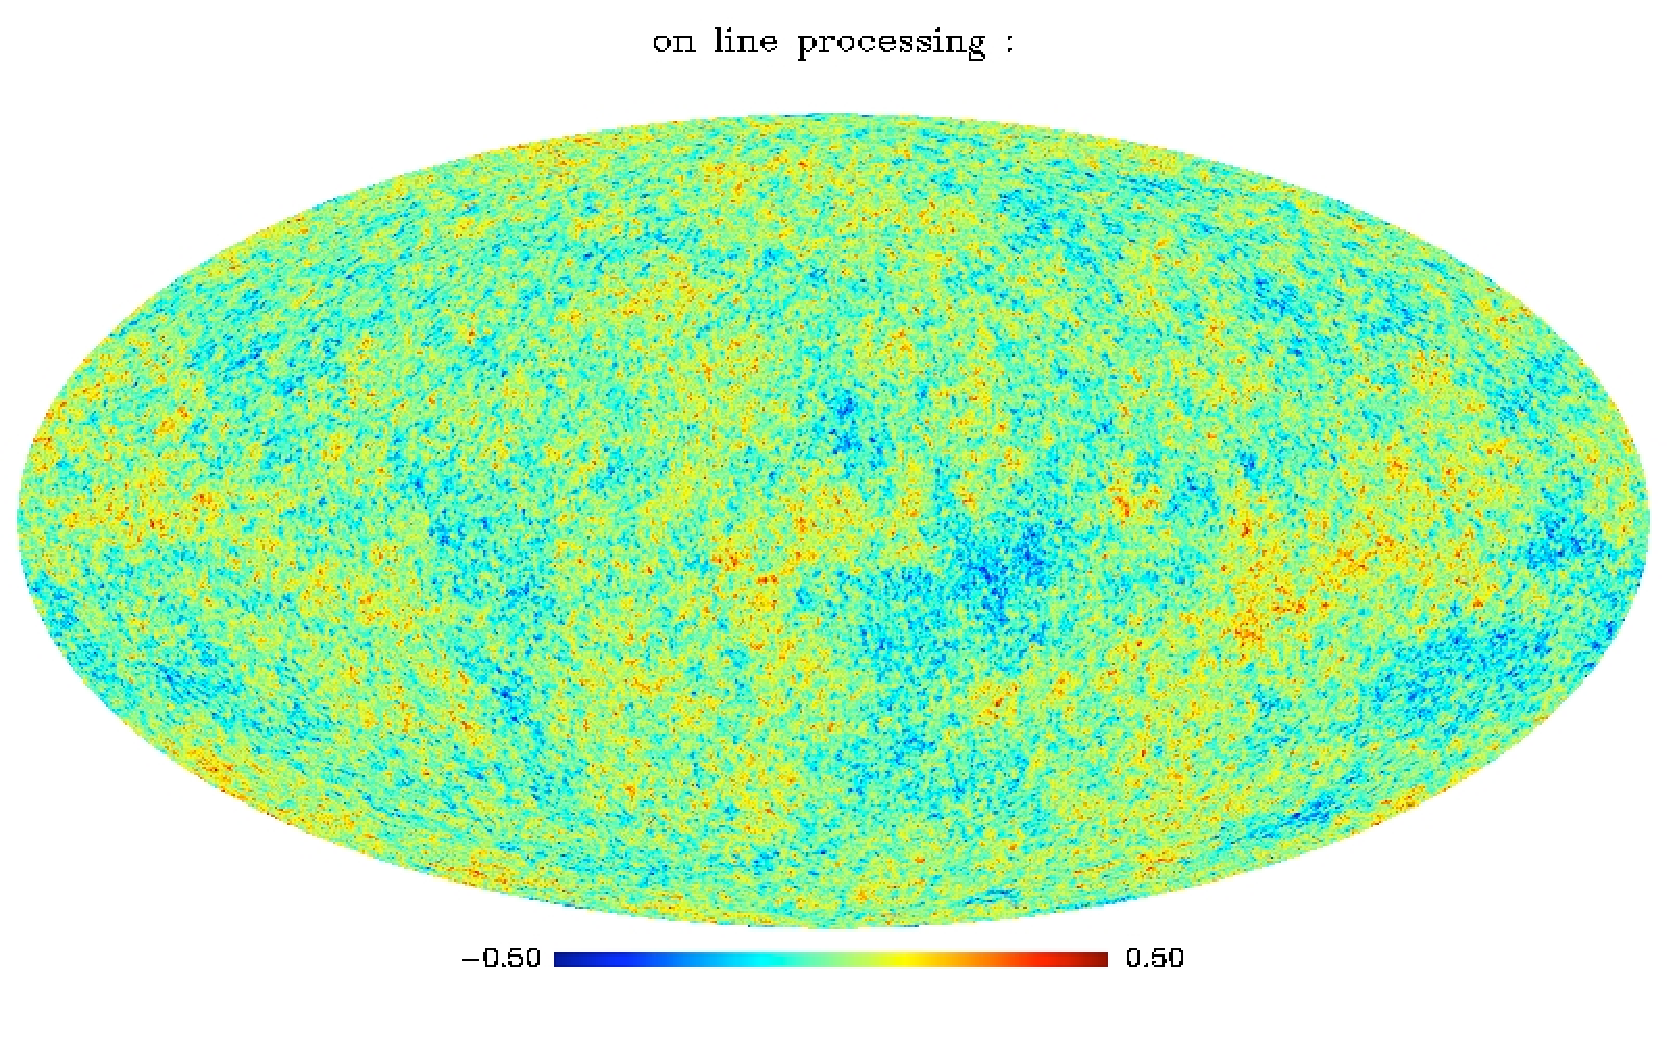
\includegraphics[width=12cm]{cmb_input.pdf} \\
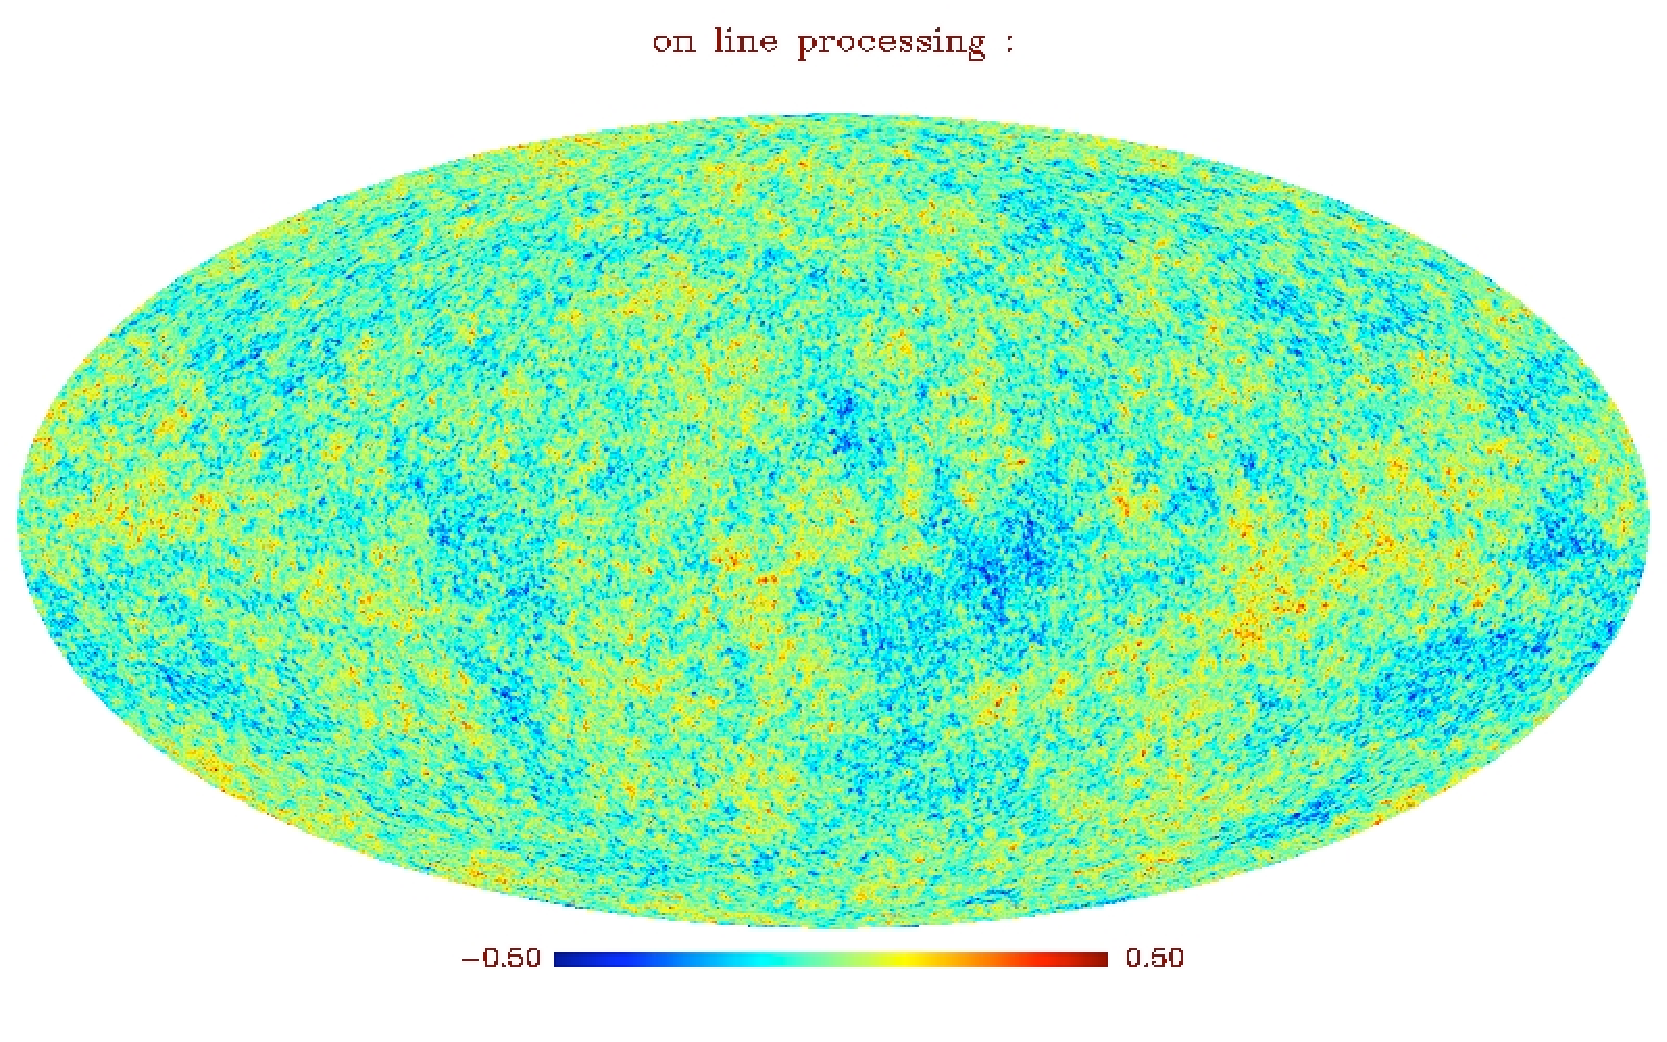
\includegraphics[width=12cm]{gmca_cmbwiener.pdf}
\end{array}
$$
\vspace{-0.1in} \caption{\textbf{Top~:} original CMB component. \textbf{Bottom~:} CMB componentestimated with GMCA. \textbf{Unit~:}  $10^{-3}$K.} \label{fig:wg2_maps}
\end{figure}
\end{center}

\begin{center}
\begin{figure}[htb]
$$
\begin{array}{cc}
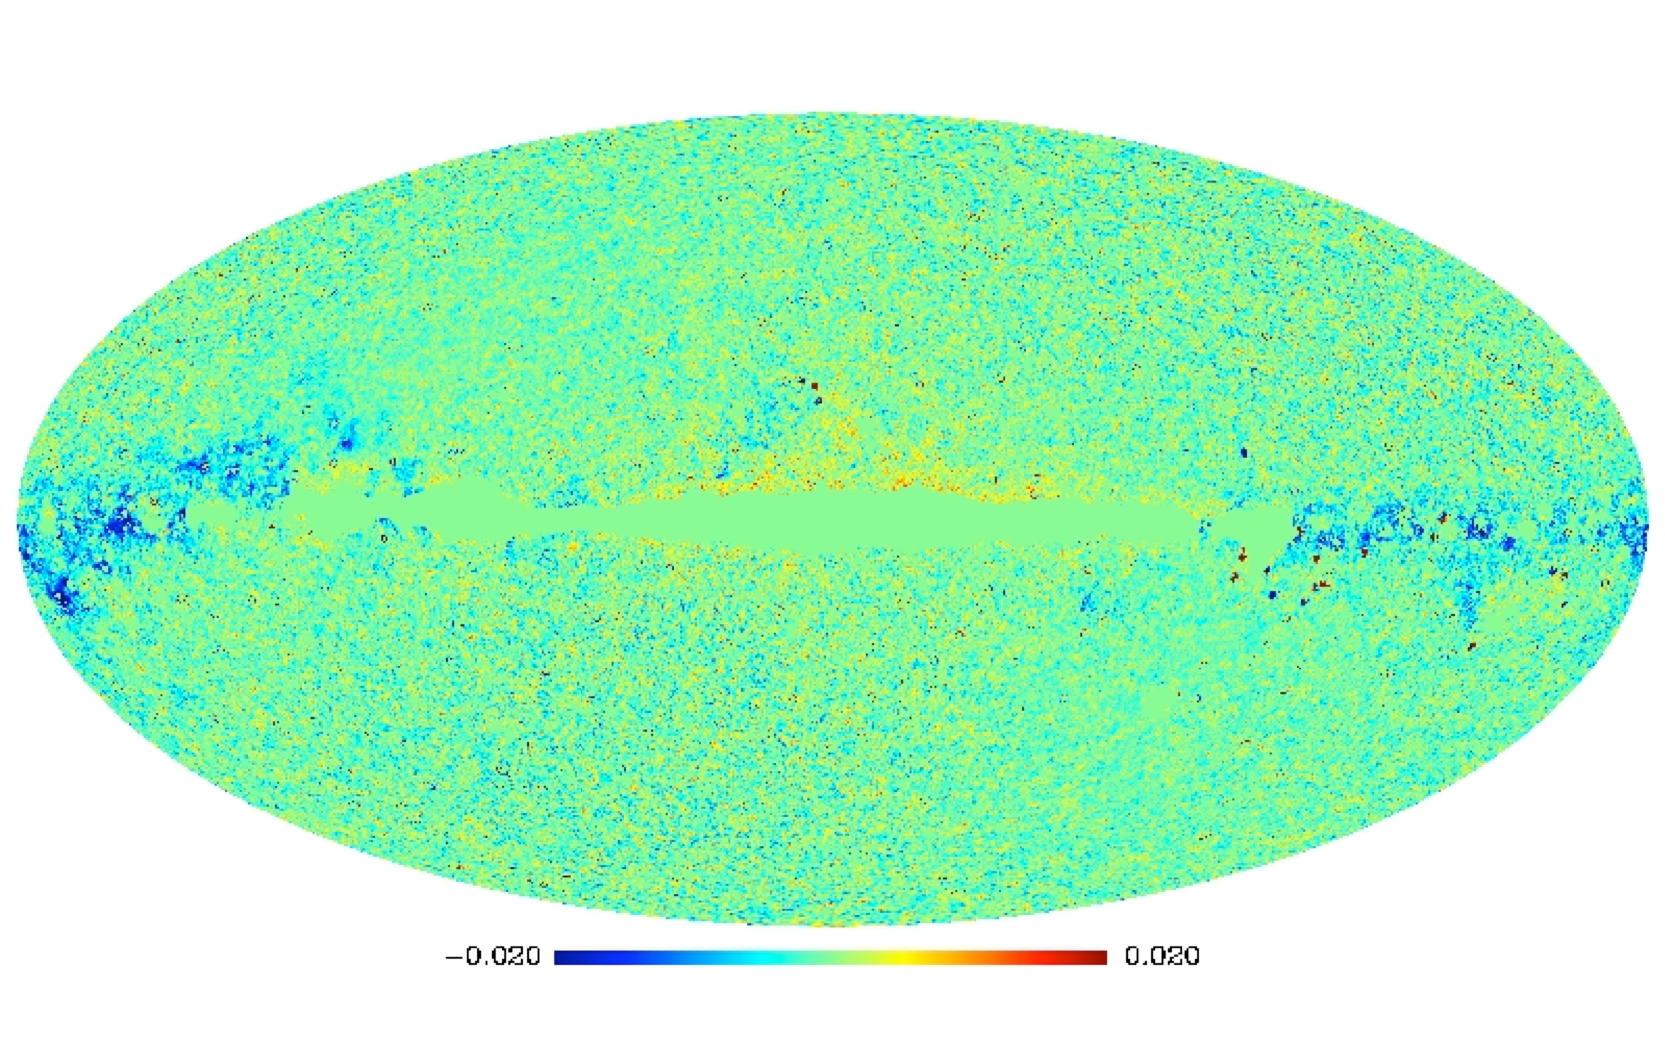
\includegraphics[width=12cm]{gmca_residual20_b.pdf} \\
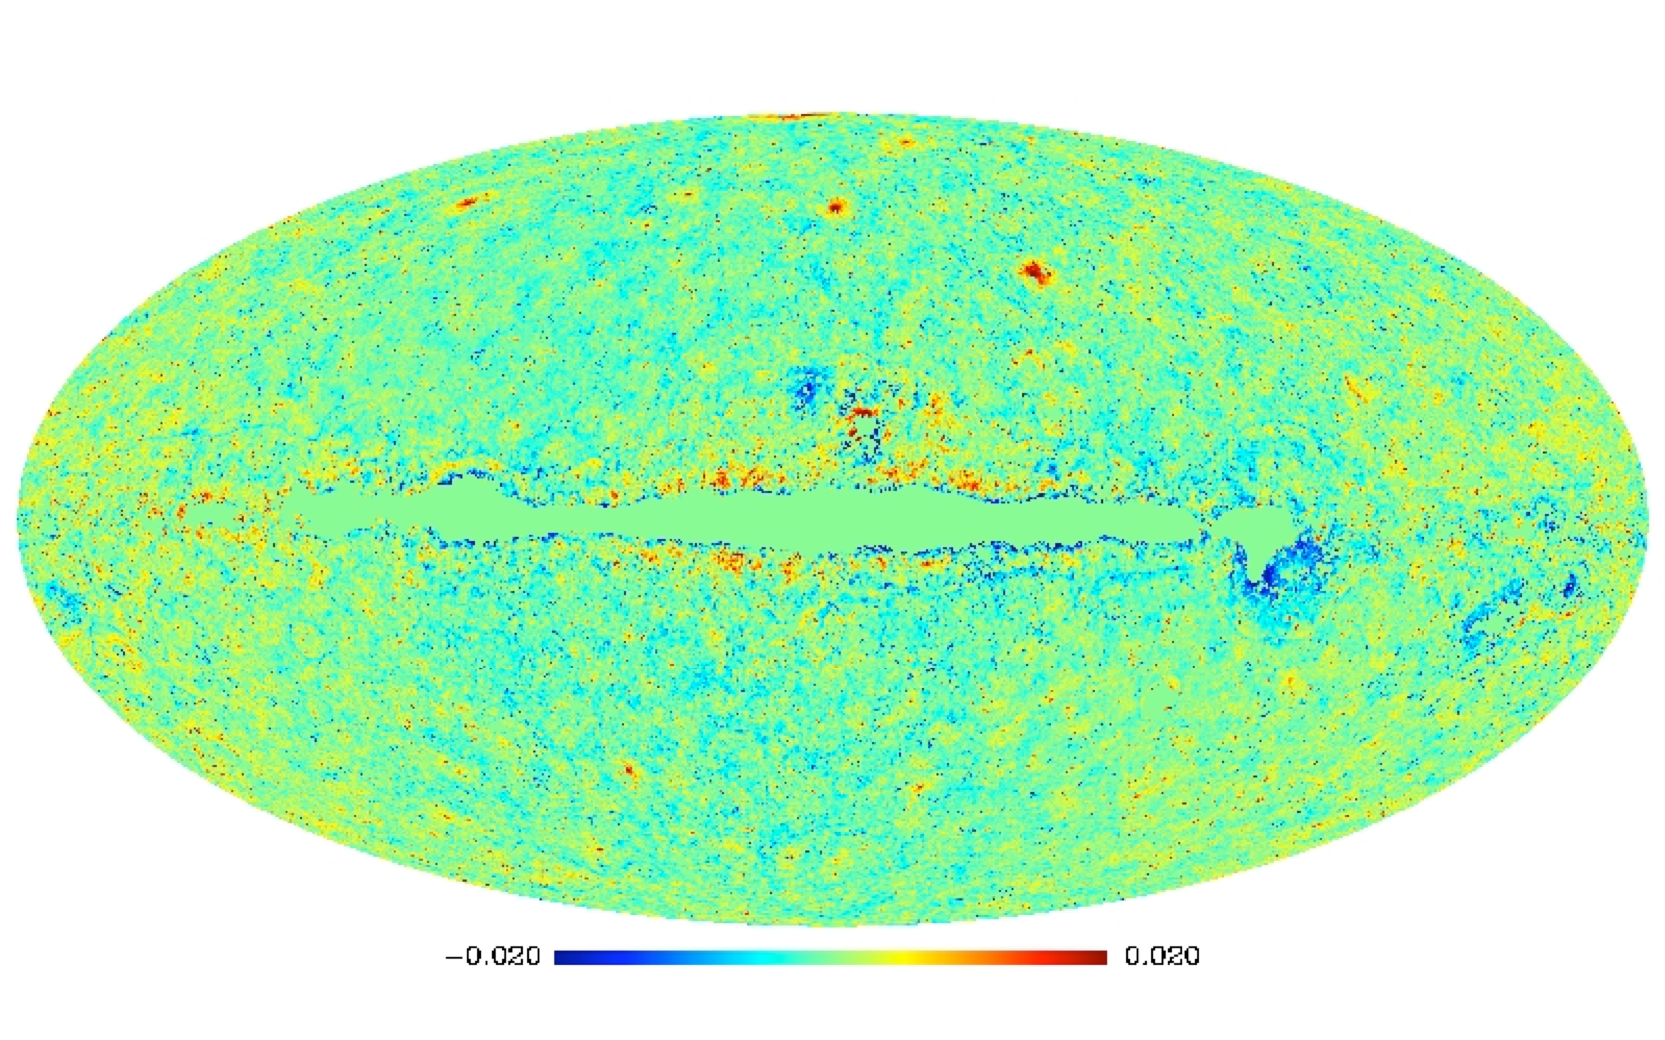
\includegraphics[width=12cm]{adamis_residual20_b.pdf} 
\end{array}
$$
\vspace{-0.1in}\caption{\textbf{Top~:} GMCA residual convolved at $20$ arcminutes. \textbf{Bottom~:} ADAMIS residual convolved at $20$ arcminutes. \textbf{Unit~:}  $10^{-3}$K.} \label{fig:wg2_resi20}
\end{figure}
\end{center}

\begin{center}
\begin{figure}[htb]
$$
\begin{array}{cc}
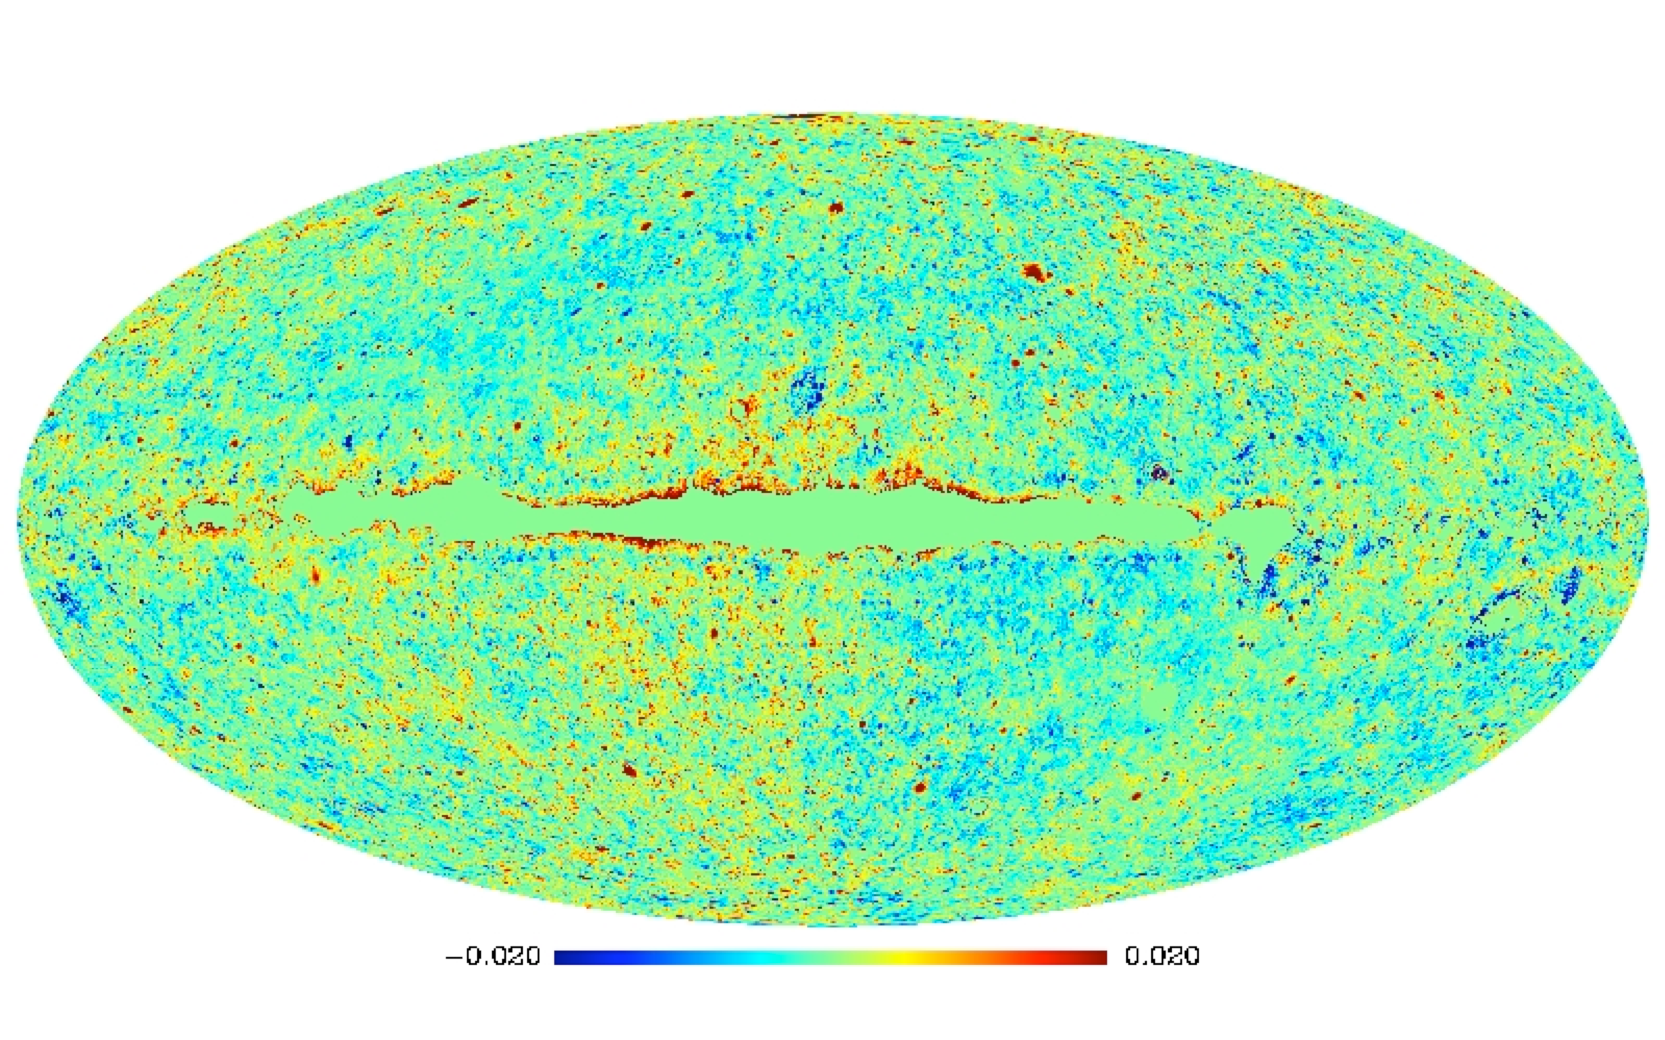
\includegraphics[width=12cm]{mem_residual20_b.pdf} \\
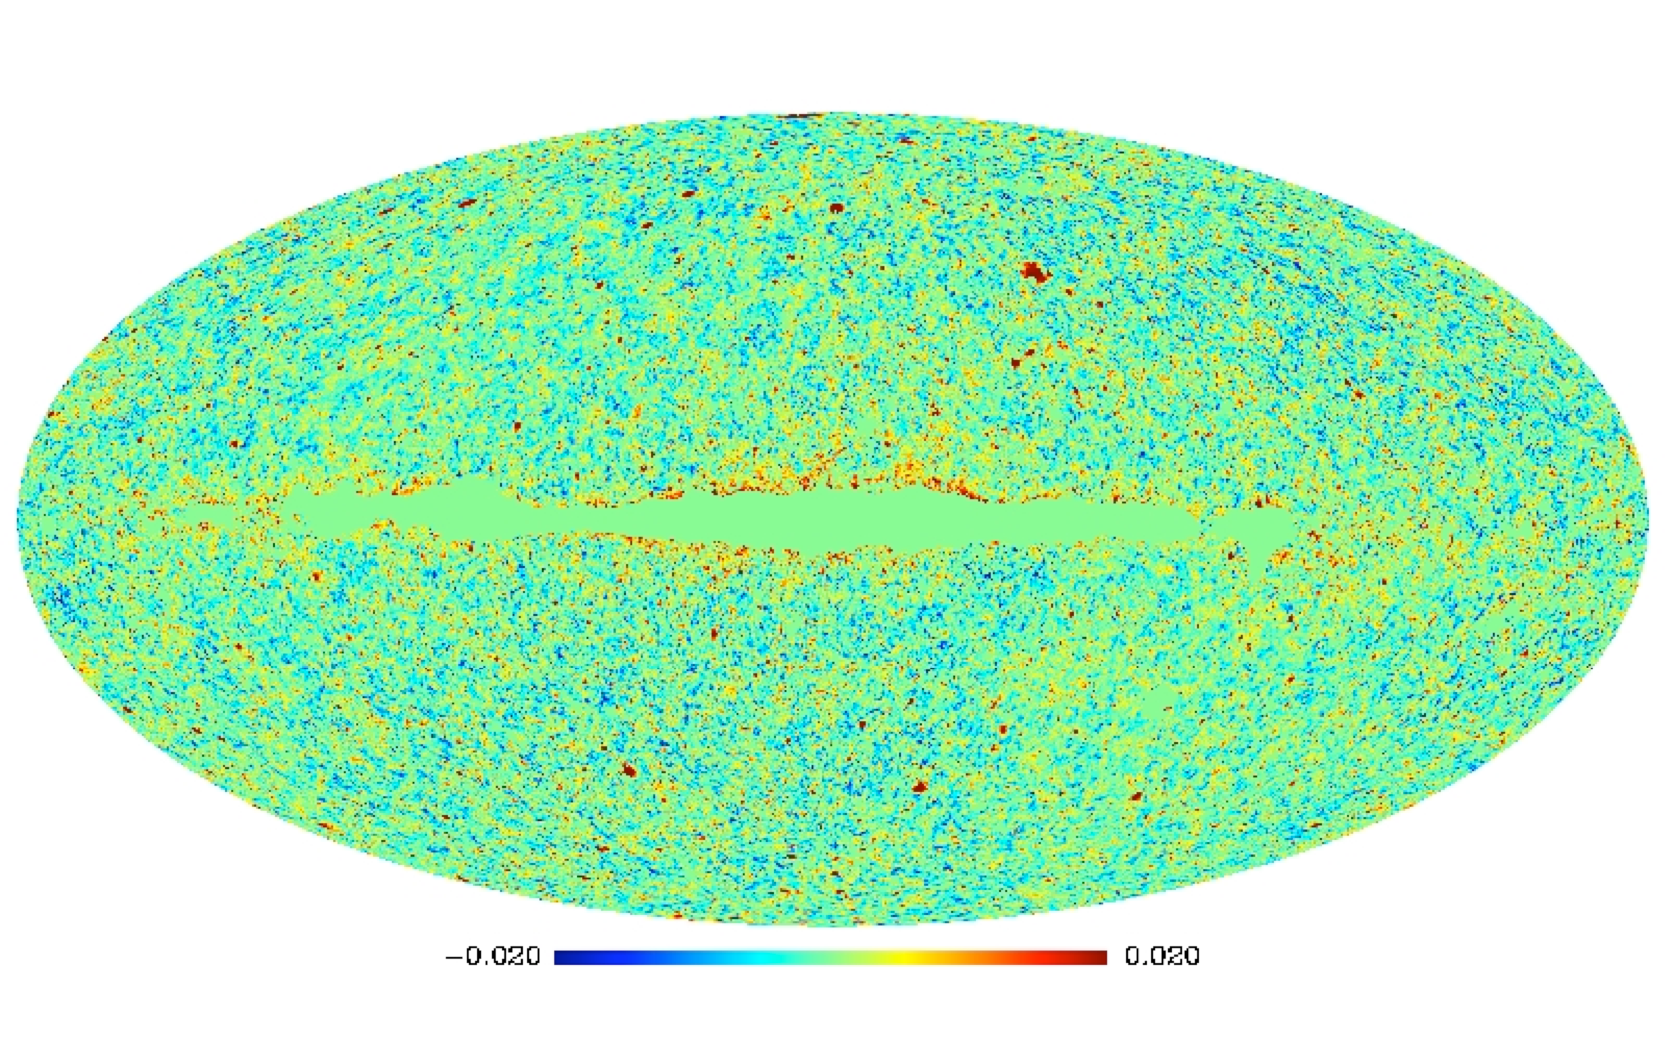
\includegraphics[width=12cm]{cca_residual20_b.pdf}
\end{array}
$$
\vspace{-0.1in} \caption{\textbf{Top~:} MEM residual convolved at $20$ arcminutes. \textbf{Bottom~:} CCA residual convolved at $20$ arcminutes. \textbf{Unit~:}  $10^{-3}$K.} \label{fig:wg2_resi20_2}
\end{figure}
\end{center}

\begin{center}
\begin{figure}[htb]
$$
\begin{array}{cc}
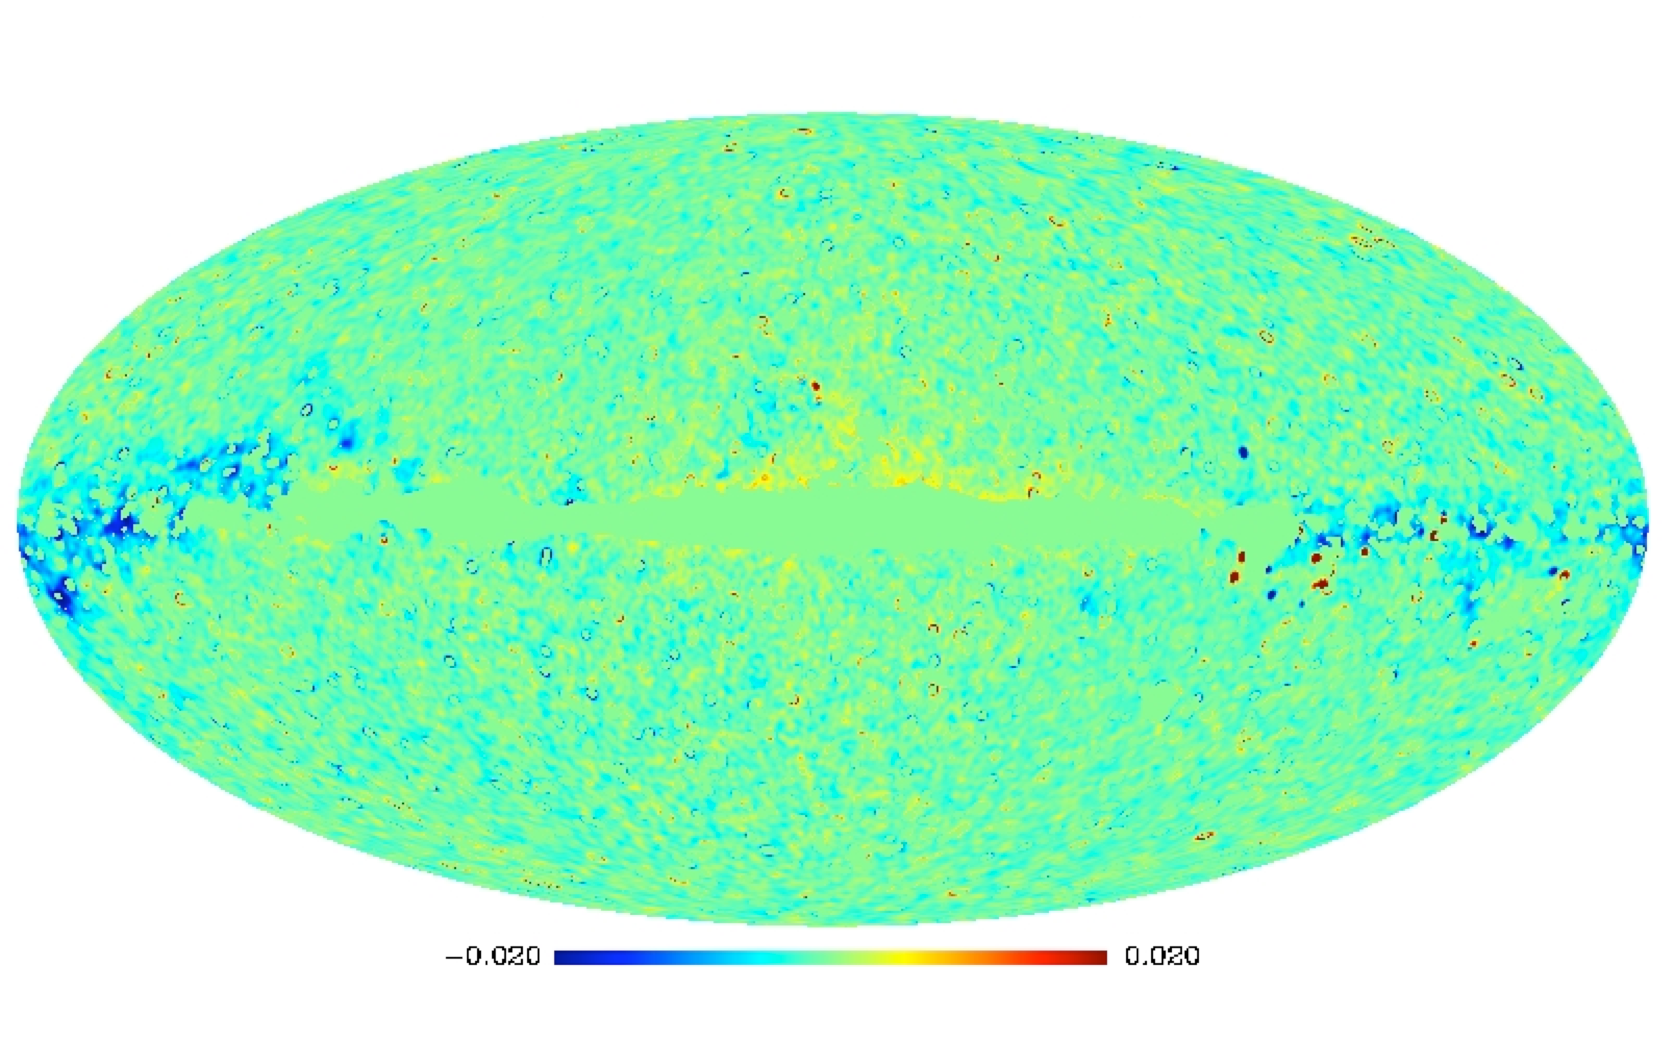
\includegraphics[width=12cm]{gmca_residual60_b.pdf} \\
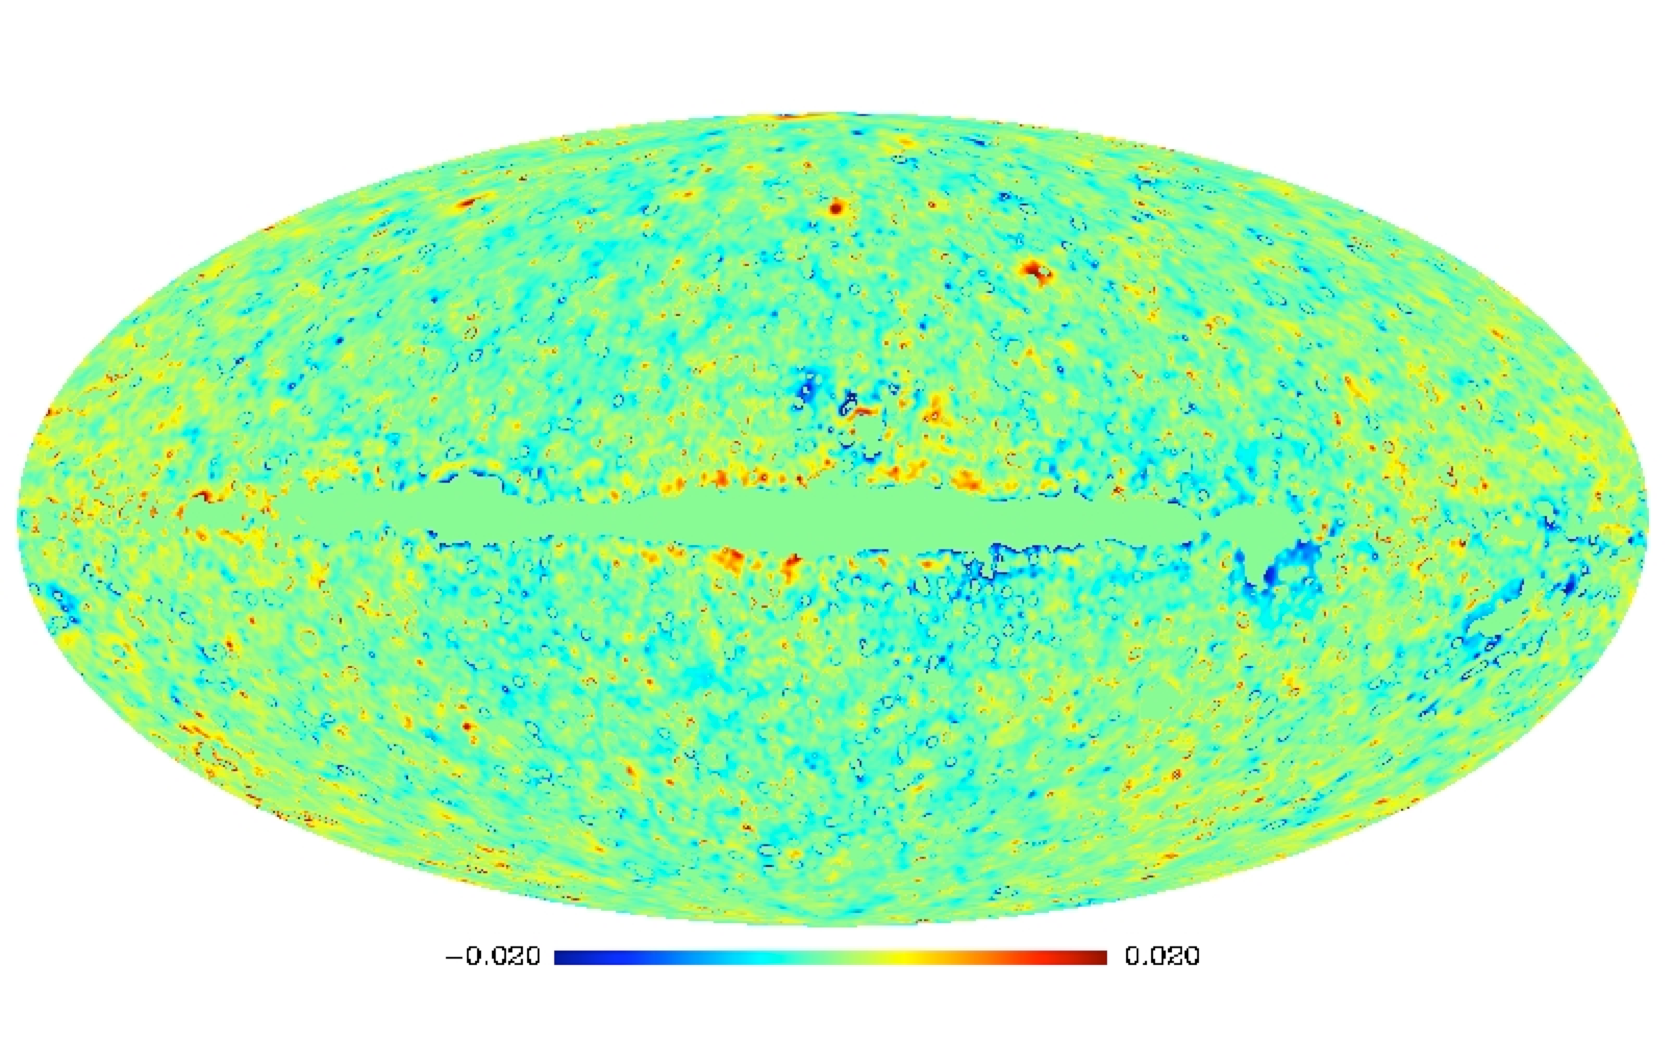
\includegraphics[width=12cm]{adamis_residual60_b.pdf} 
\end{array}
$$
\vspace{-0.1in} \caption{\textbf{Top~:} GMCA residual convolved at $60$ arcminutes. \textbf{Bottom~:} ADAMIS residual convolved at $60$ arcminutes. \textbf{Unit~:}  $10^{-3}$K.} \label{fig:wg2_resi60}
\end{figure}
\end{center}

\begin{center}
\begin{figure}[htb]
$$
\begin{array}{cc}
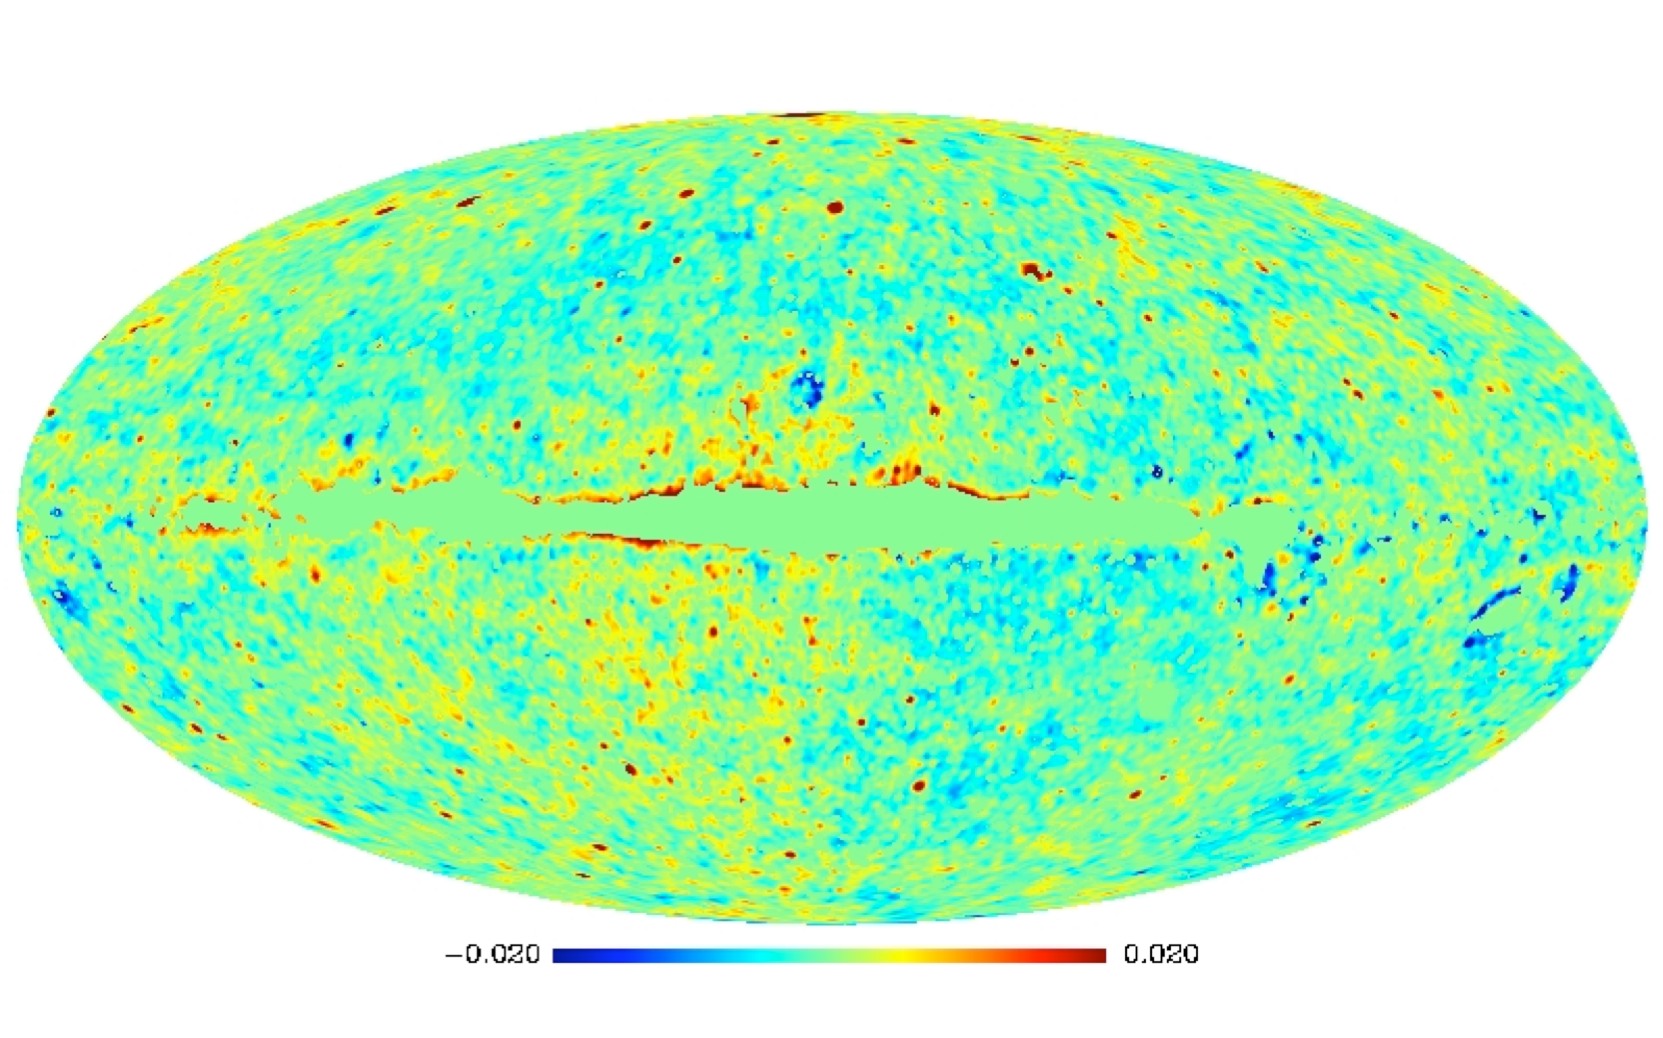
\includegraphics[width=12cm]{mem_residual60_b.pdf} \\
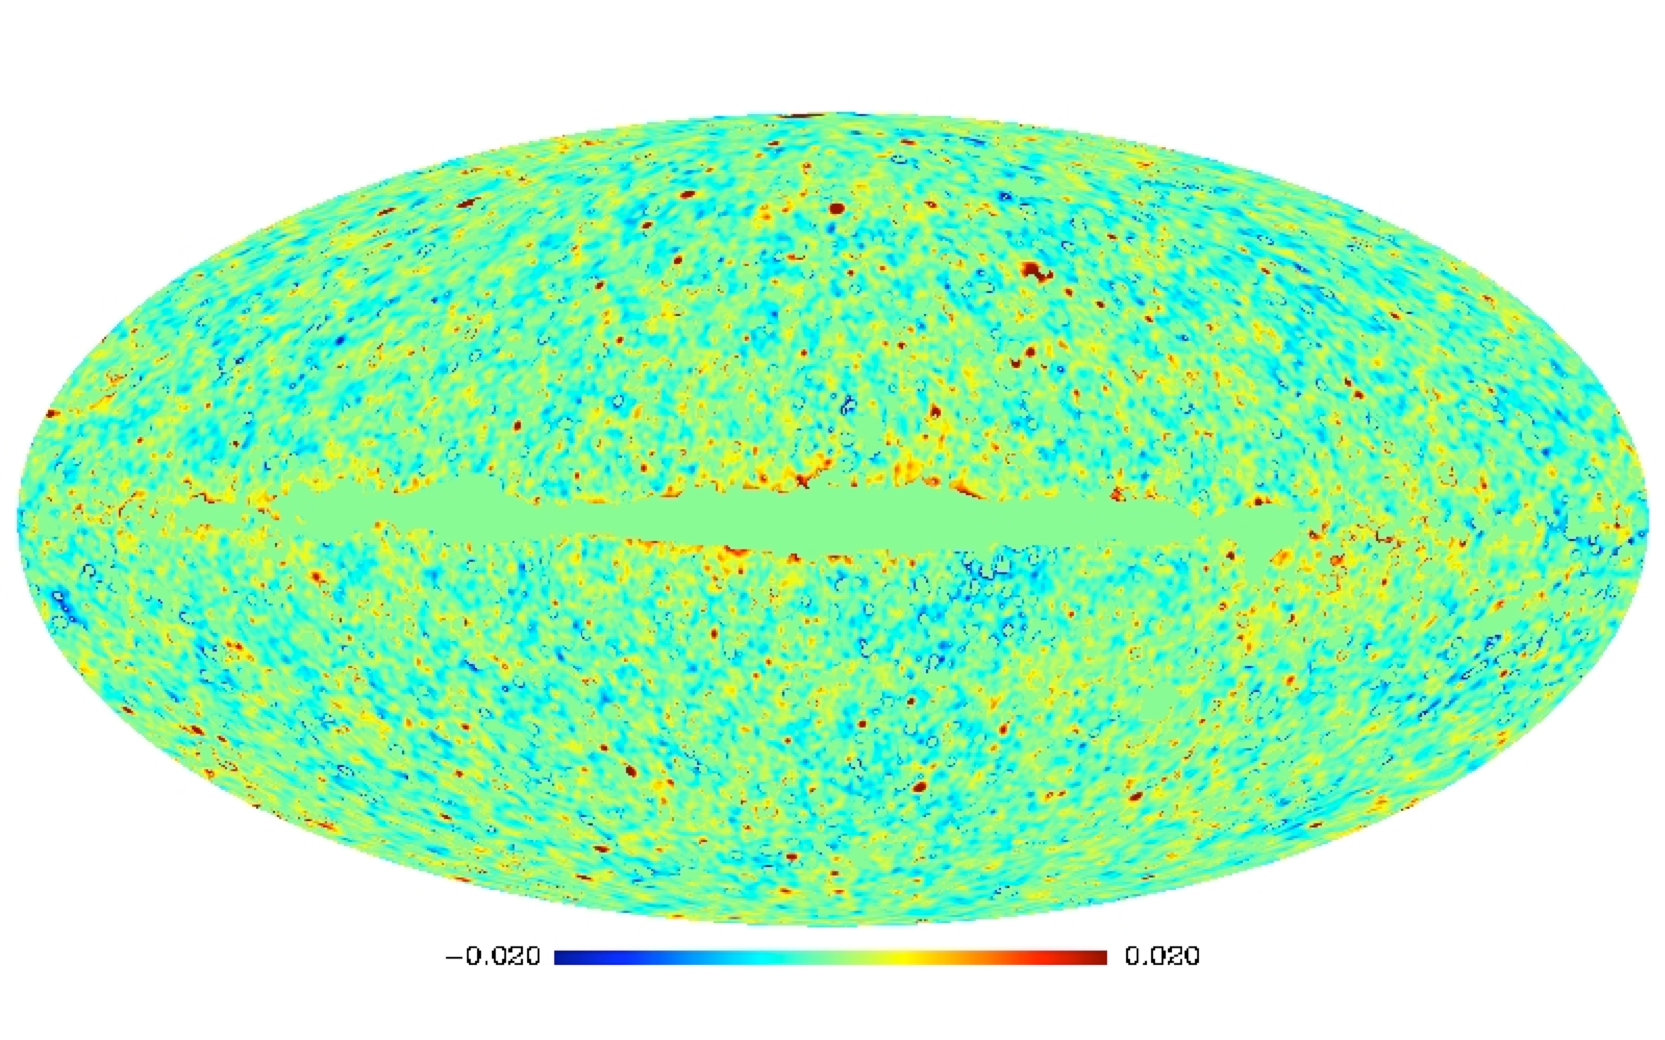
\includegraphics[width=12cm]{cca_residual60_b.pdf}
\end{array}
$$
\vspace{-0.1in} \caption{\textbf{Top~:} MEM residual convolved at $60$ arcminutes. \textbf{Bottom~:} CCA residual convolved at $60$ arcminutes. \textbf{Unit~:}  $10^{-3}$K.} \label{fig:wg2_resi60_2}
\end{figure}
\end{center}

\begin{figure}[htb]
\hspace{0.1in}
$$
\begin{array}{c}
%\begin{minipage}[b]{1\linewidth}
    \centerline{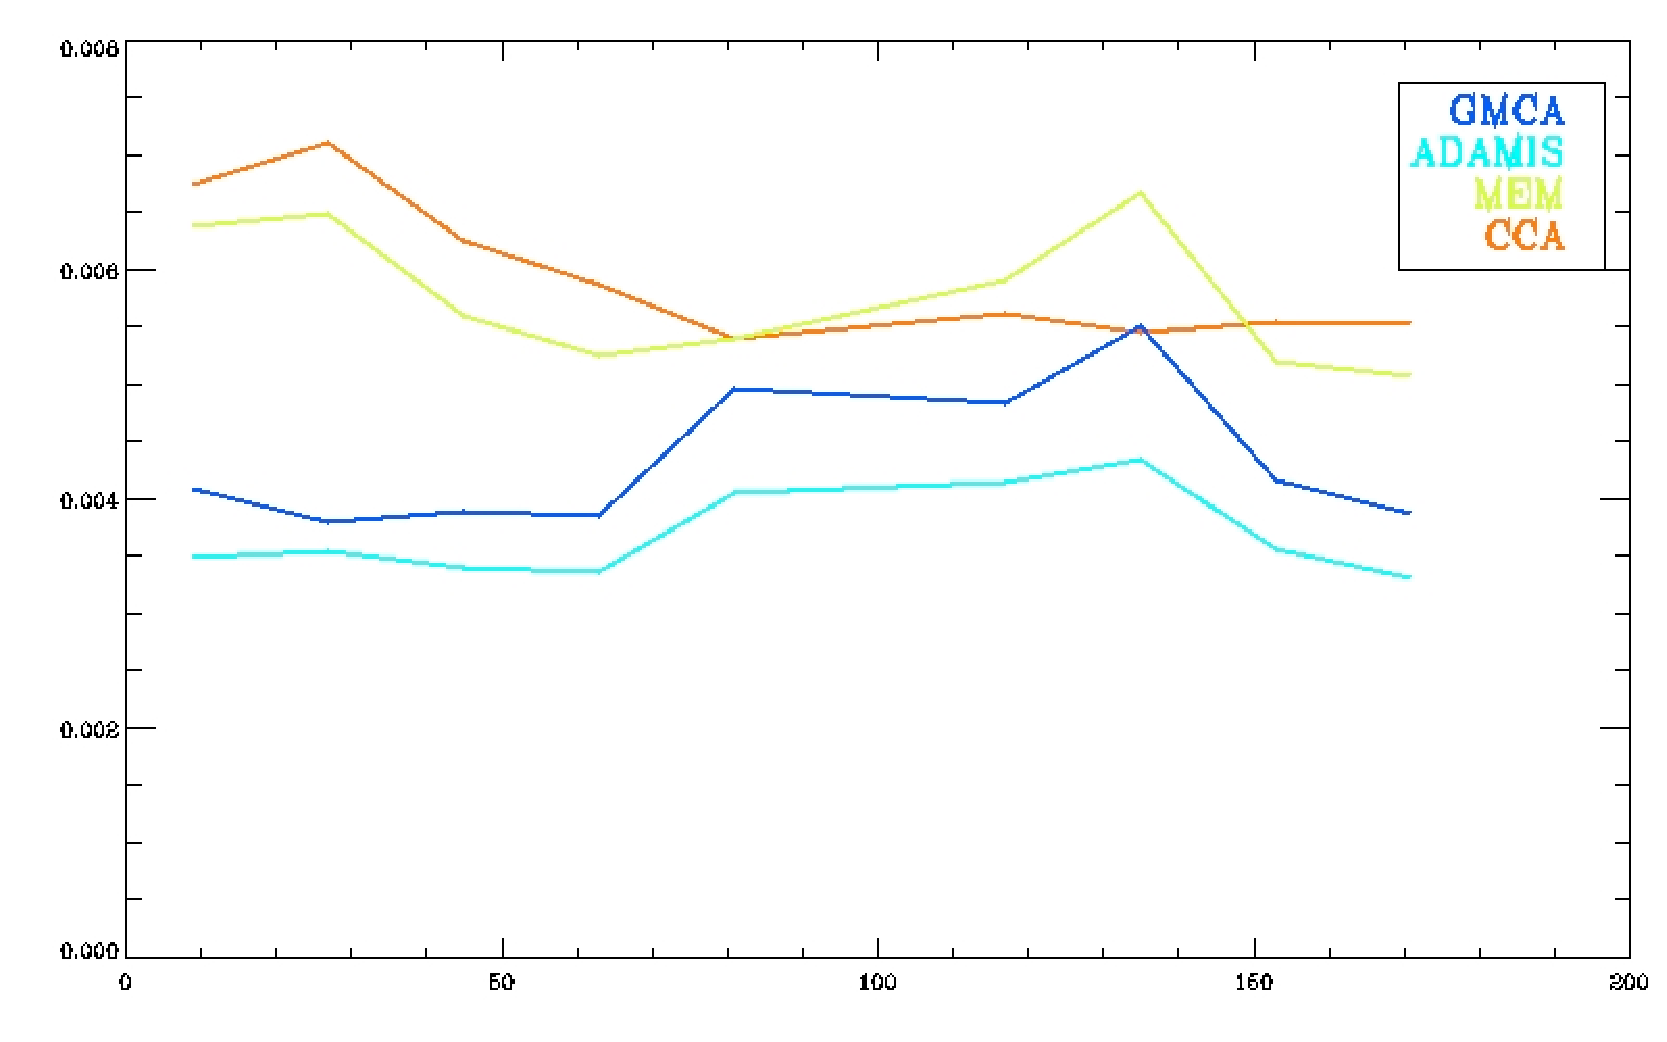
\includegraphics[width=12cm]{Residual_per20deg_20arcm.pdf}} \\
%\end{minipage}
%\vfill
%\begin{minipage}[b]{1\linewidth}
    \centerline{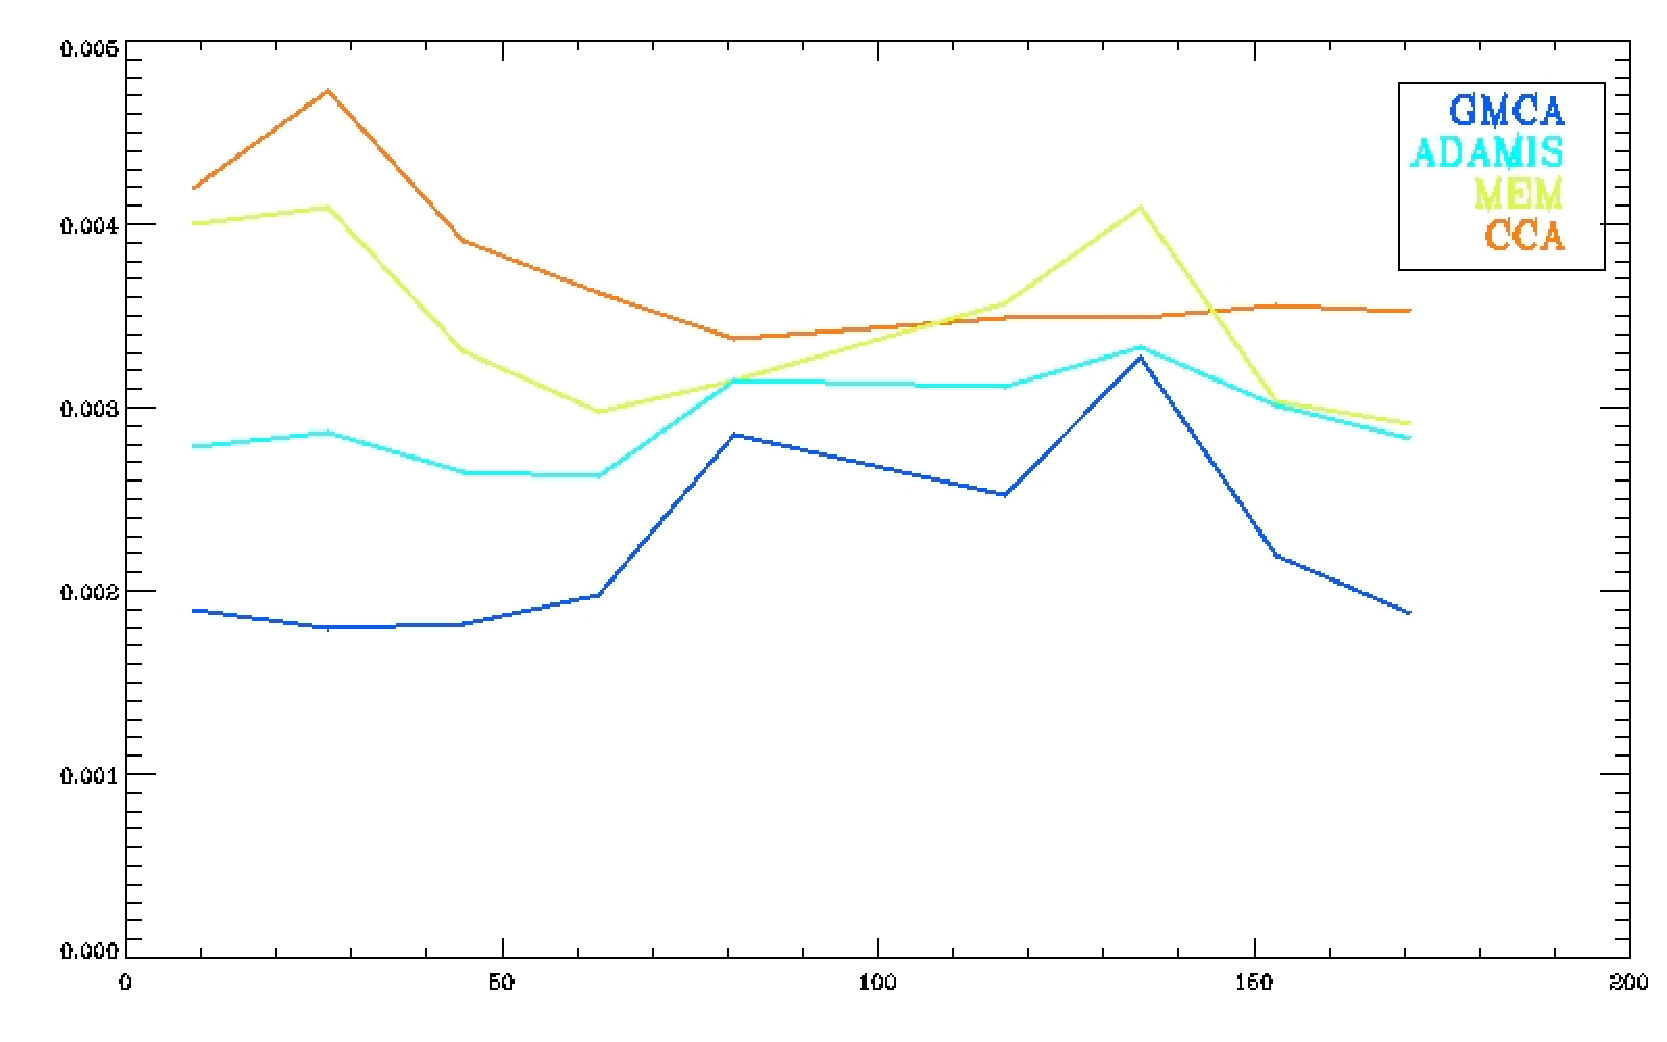
\includegraphics[width=12cm]{Residual_per20deg_60arcm.pdf}}
%\end{minipage}
\end{array}
$$
\vspace{-0.1in} 
\caption{\textbf{Top~:} standard deviation of the residual convolved at $20$ arcminutes per latitude bands with a width of $20^\circ$.\textbf{Bottom~:} standard deviation of the residual convolved at $60$ arcminutes per latitude bands with a width of $20^\circ$. \textbf{Abscissa~:} central latitude. The band centered in $90^\circ$ is not plotted. \textbf{Up~:} standard deviation of the residual in mK.}  \label{fig:wg2_resiperlat}
\end{figure}

